\documentclass[a4paper, 12pt]{article}
\usepackage{../sty/sbl-annual-meeting}
\title{{\Large\titlefont The CBGM: An Illustrated Crash Course}\\{\large\titlefont\color{HokieStone}Supplement to ``The open-cbgm Library: Design and Demonstration''}}
\author{{\normalsize\sf\textsc{Joey McCollum}}\\{\normalsize\sf Virginia Polytechnic Institute and State University}\\{\normalsize\sf\url{jjmccollum@vt.edu}}}
\date{{\normalsize\sf 21–24 November 2020}}
\begin{document}
	\maketitle
	\section*{Introduction}
	This document presents a brief introduction to the Coherence-Based Genealogical Method (CBGM), organized around the core elements of the method. For didactic purposes, key concepts are introduced primarily through graphics and practical examples; for more in-depth technical discussion, interested readers are encouraged to consult any of the comprehensive treatments of the CBGM in the literature.\footnote{See \cite{Mink04}; \cite{Gurry16}; \cite{WG17}; and \cite{Gurry17}. An extensive, amply illustrated introductory presentation by Gerd Mink is accessible at \url{https://www.uni-muenster.de/INTF/cbgm_presentation/download.html}.} Basic knowledge of textual criticism is assumed, but readers new to the CBGM should be able to follow this presentation with no other prior knowledge. Familiarity with New Testament Greek is necessary to understand the content of textual variants in some examples, but not necessary to understand how the CBGM treats variants, as the CBGM works independently of the language of the text to which it is applied.\footnote{While the CBGM has been most widely adopted for the study of the Greek New Testament, it has also been employed in the study of the Hebrew Bible; see \cite{Ellis18}.}
	
	\section{Local Stemmata}\label{sec:local-stemmata}
	The basic unit of comparison in the CBGM is the \emph{local stemma of variant readings}. 
	
	\begin{wrapfigure}{r}{0.5\textwidth}
		\vspace{-\baselineskip}
		\centering
		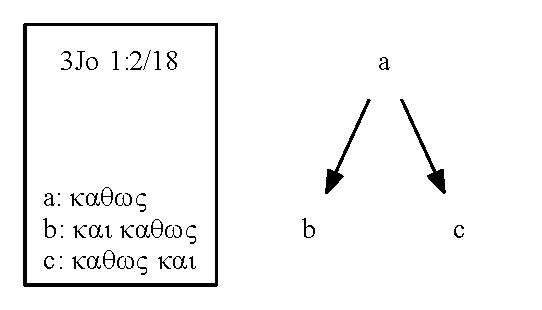
\includegraphics[scale=0.6666]{../graphics/B25K1V2U18-local-stemma.pdf}
		\caption{A local stemma of readings (3~John 1:2\ForwardSlash 18). Here, reading \emph{a} is judged to be the initial reading, and it is posited to have given rise to readings \emph{b} and \emph{c}.}
		\label{fig:local-stemma}
		\vspace{\baselineskip}
		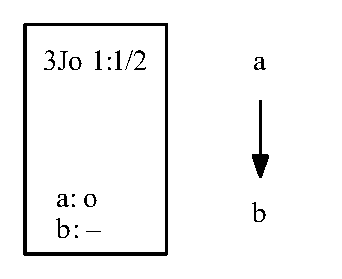
\includegraphics[scale=0.6666]{../graphics/B25K1V1U2-local-stemma.pdf}
		\caption{A simple local stemma (3~John 1:1\ForwardSlash 2).}
		\label{fig:local-stemma-simple}
	\end{wrapfigure}
	\noindent
	A local stemma is a graphical representation of text-critical judgments about competing readings in a portion of the text. Readings are represented by nodes in the stemma, and their hypothesized relationships are represented by directed edges (see Fig.~\ref{fig:local-stemma}). Local stemmata are traditionally indexed by the units where the textual variation occurs. The number or numbers occurring after the ``\ForwardSlash '' in the index refer to word indices in the base text. Each word in the base text is assigned an even number, while spaces in between words (for variant readings that are additions not found in the base text) are assigned odd numbers. 
	
	%The criterion of intrinsic probability (``which reading most coheres with the author's perceived style, purpose, audience, cultural context, etc.?''), if it is sufficiently strong, can determine the root of the local stemma. The criterion of transcriptional probability (``which readings likely gave rise to others on the basis of scribal habits and motivations?'') governs the placement of the edges in the stemma. External evidence (``which readings have the earliest or most widespread attestation?'') also sheds light on how the local stemma should be oriented.
	%Consider the stemma in Fig.~\ref{fig:local-stemma}. Reading \emph{a} is placed at the root of the local stemma due to its relative simplicity and its near-unanimous support in the surviving manuscript tradition. Readings \emph{b} and \emph{c} can be explained as small additions made to reading \emph{a} in anticipation of another infinitive after the first two or in the interest of strengthening the connection between the two phrases surrounding this textual variation; therefore, the stemma features edges from reading \emph{a} to each of these readings.
	
	Most local stemmata are simple, like the one pictured in Fig.~\ref{fig:local-stemma-simple}. In most cases where there are two variant readings, one is sparsely attested or obviously secondary, and orienting the local stemma is straightforward.
	
	\newpage
	
	For reasons we will discuss later, a desirable property of a local stemma is that it has a reading from which we can reach all other readings in the stemma. We will refer to this property as \emph{completeness}. In practical terms, a complete local stemma is one in which every reading can be explained, either as the earliest reading or as a later reading derived from a known earlier reading. The concept is illustrated in Fig.~\ref{fig:local-stemma-complete}.
	
	\begin{figure}[h!]
		\centering
		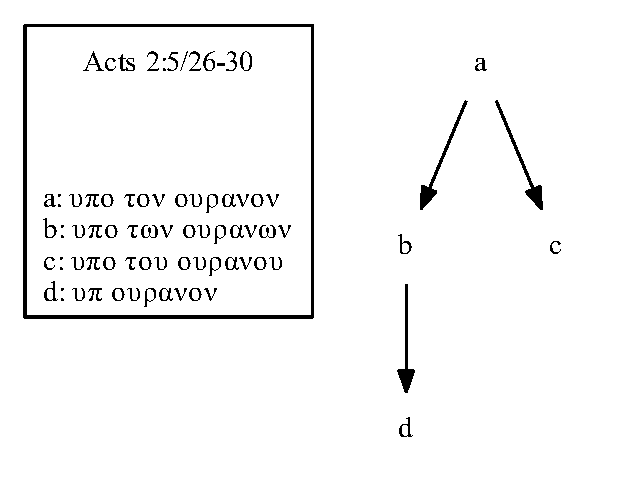
\includegraphics[scale=0.6666]{../graphics/B05K2V5U26-30-local-stemma.pdf}\\
		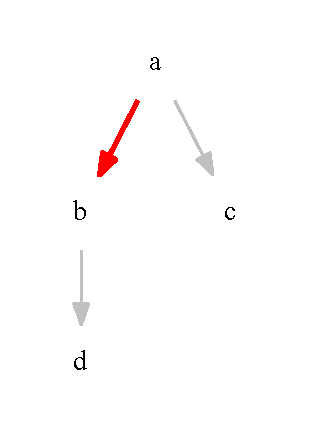
\includegraphics[scale=0.6666]{../graphics/B05K2V5U26-30-local-stemma-path-1.pdf}
		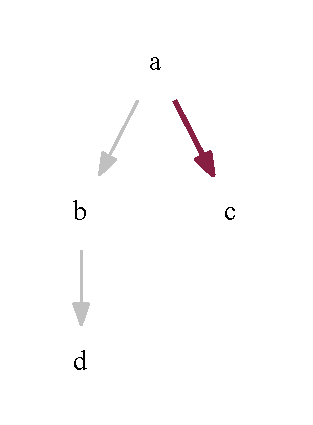
\includegraphics[scale=0.6666]{../graphics/B05K2V5U26-30-local-stemma-path-2.pdf}
		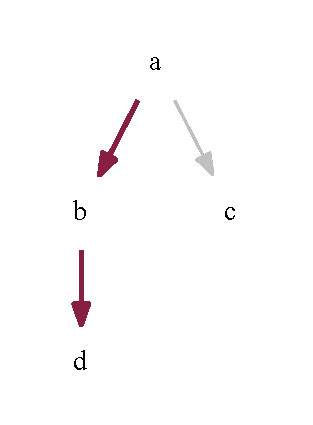
\includegraphics[scale=0.6666]{../graphics/B05K2V5U26-30-local-stemma-path-3.pdf}
		\caption{A complete local stemma (Acts 2:5\ForwardSlash 26–30). This stemma is complete because there is a path from reading \emph{a} to every other reading.}
		\label{fig:local-stemma-complete}
	\end{figure}
	
	\newpage
	
	An example of an incomplete stemma appears in Fig.~\ref{fig:local-stemma-incomplete}. This local stemma also exhibits some additional features that arise from editorial judgment. The reading \emph{af} represents a \emph{defective subvariant} of reading \emph{a}, meaning that the editors considered it a nonsense reading that originated from reading \emph{a}. (The \emph{f} suffix stands for \emph{Fehler}, the German word for \emph{error}.) \emph{Orthographic subvariants} (not pictured here), which involve known differences in spelling conventions, are also common; they are denoted using the \emph{o} suffix. The reading \emph{d2} represents a \emph{split attestation} of reading \emph{d}; the editors thought that the same reading arose two times independently, and so they split it into two identical readings for the purpose of genealogical analysis. Finally, reading \emph{zw-a\ForwardSlash b} represents an \emph{ambiguous reading}, which, due to damage or gaps in one or more manuscripts, was difficult to make out and could represent any one of multiple readings.
	
	In this example, we have highlighted the edges ending at readings \emph{af} and \emph{zw-a\ForwardSlash b} with dashed lines because these types of readings are typically not included in local stemmata. In practice, defective and orthographic subvariants are usually merged with their parent readings for the purpose of comparison, and ambiguous readings are treated as lacunae and dropped from the stemma entirely. More importantly, there is no edge that connects reading \emph{d2} to the rest of the stemma because the editors were uncertain about the origin of this reading.
	
	\begin{figure}[h!]
		\centering
		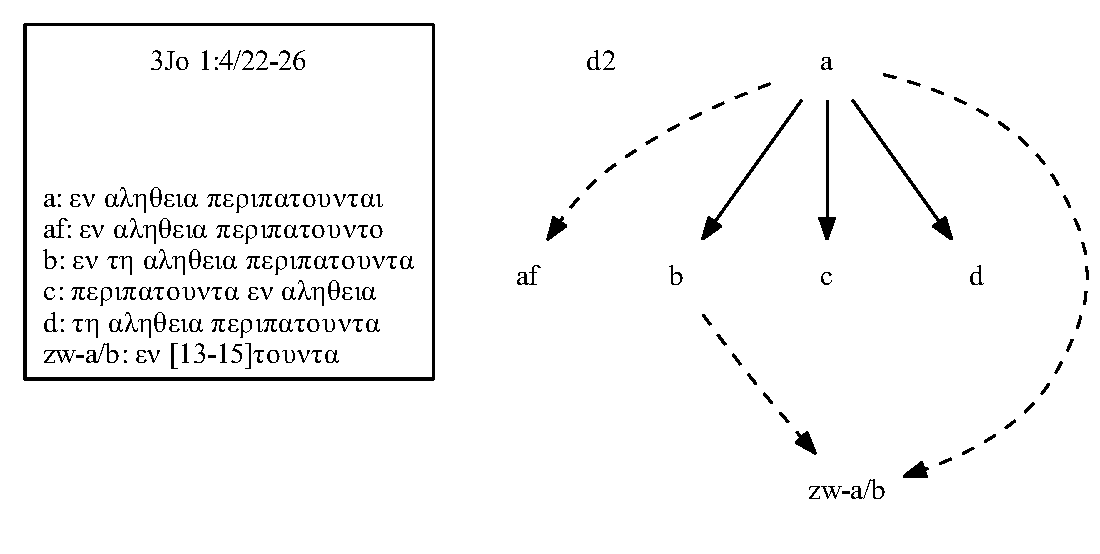
\includegraphics[scale=0.6666]{../graphics/B25K1V4U22-26-local-stemma.pdf}
		\caption{An incomplete local stemma (3~John 1:4\ForwardSlash 22–26).}
		\label{fig:local-stemma-incomplete}
	\end{figure}
	
	\newpage
	
	The incomplete stemma in Fig.~\ref{fig:local-stemma-complex} is even more complicated. Here, variant readings abound (even after we ignore subvariants, split attestations, and ambiguities!), and there are many potential relationships that are not certain. At least four readings could have given rise to the omission in reading \emph{i}, but on the basis of intrinsic and transcriptional factors alone, it is unclear which reading or readings are most likely. Often, textual critics must revise local stemmata on the basis of genealogical relationships between witnesses that support different readings. Section \ref{sec:textual-flow} will show how this is done in the CBGM.
	
	\begin{figure}[h!]
		\centering
		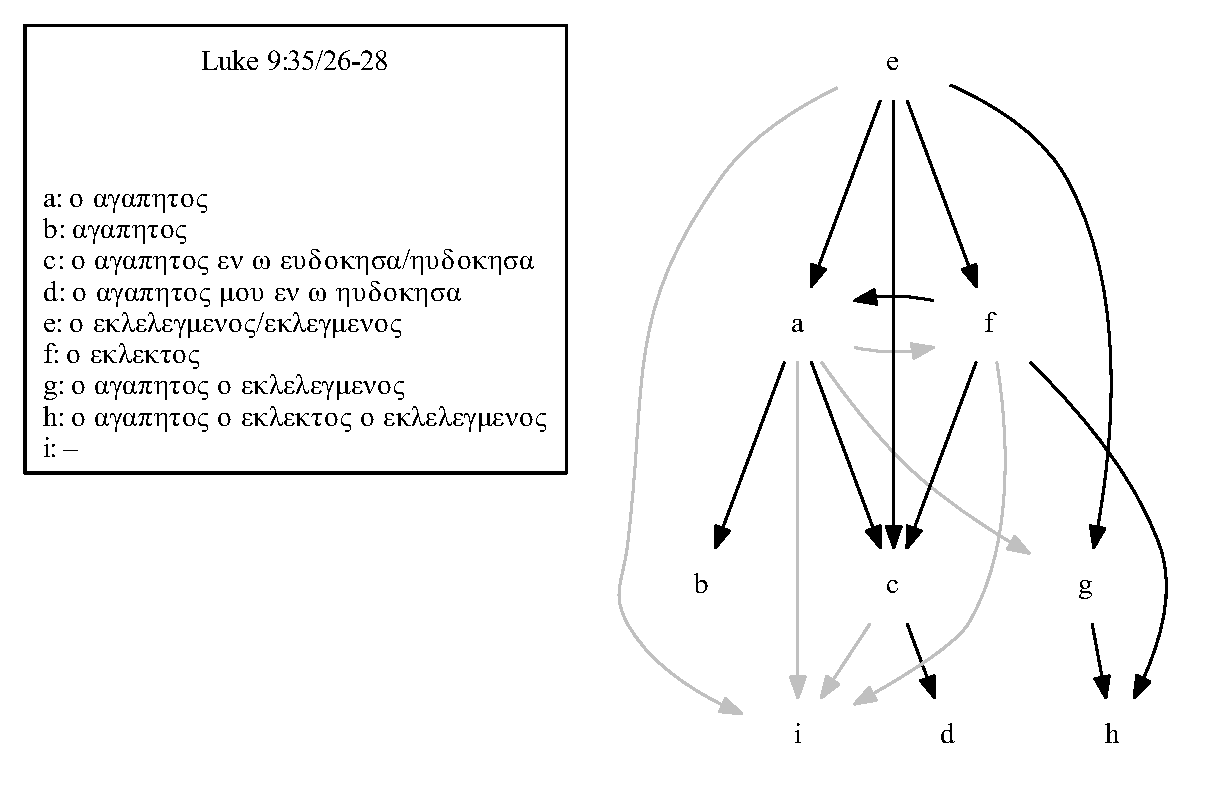
\includegraphics[scale=0.6666]{../graphics/B03K9V35U26-28-local-stemma.pdf}
		\caption{A more complex incomplete local stemma (Luke 9:35\ForwardSlash 26–28) with potential, but uncertain relationships highlighted in gray, adapted from \cite{McCollum20}. For the sake of space, subvariants and potential split attestations have been merged with their parent readings. In practice, splits should be introduced to prevent loops (like the one between \emph{a} and \emph{f}) and to avoid confusion between conflate readings with multiple sources (\emph{h} and possibly \emph{g}) and readings that likely arose multiple times independently (\emph{a}, \emph{c}, and possibly \emph{i}).}
		\label{fig:local-stemma-complex}
	\end{figure}
	
	\newpage
	
	\section{Textual Witnesses and Their Relationships}\label{sec:witnesses}
	Functionally speaking, a \emph{witness} is a set of variant readings.

	\begin{figure}[h!]
		\centering
		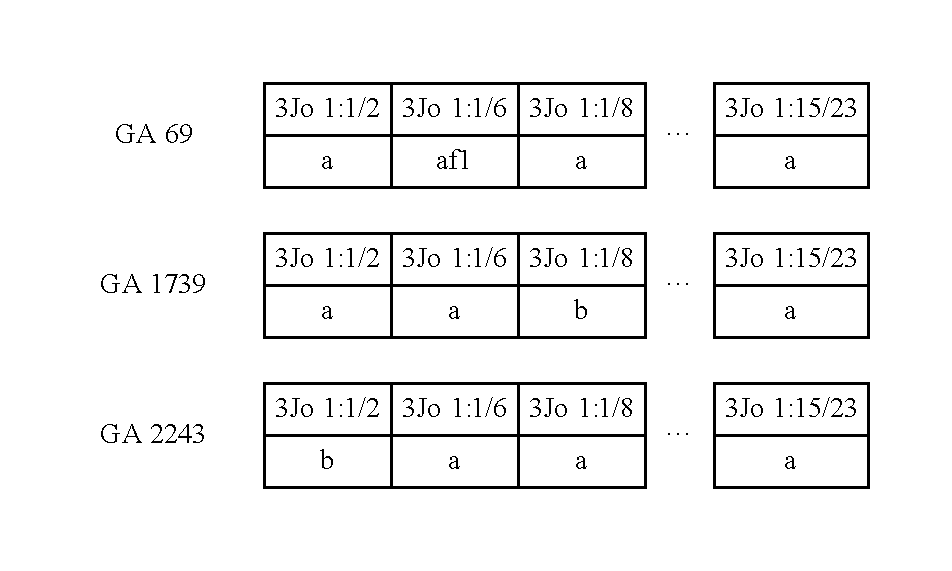
\includegraphics[scale=0.6666]{../graphics/witnesses.pdf}
		\caption{A graphical representation of three witnesses as sets of readings.}
		\label{fig:witnesses}
	\end{figure}
	\noindent
	Traditional textual criticism aims to retrace the textual history of a work in terms of documentary evidence (e.g., manuscripts, translations, and citations), making use of hypothetical ancestors to explain the common features found in surviving evidence. The CBGM departs from this model by rejecting the use of hypothetical ancestors and instead describing textual history solely in terms of abstract ``textual states'' attested by surviving evidence. The use of witnesses (as defined above) in lieu of manuscripts simplifies the problem greatly, as it removes questions of manuscript age and provenance from the reconstruction of textual history.\footnote{For more detailed discussion of this aspect of the CBGM, see \cite{Wachtel15} and \cite{Carlson15}.}
	
	\newpage
	
	\subsection{The Initial Text}\label{subsec:initial-text}
	There is one exceptional witness that is not derived from surviving evidence: the \emph{initial text}. Following the usual convention, we will denote it by the siglum \emph{A} (for the German \emph{Ausgangstext}). This special witness consists of all readings deemed the earliest in their respective local stemmata. If editors cannot decide on an earliest reading in a passage, then the initial text is treated as lacunose in that passage. Alternatively, editors may prefer a conjectural reading not found in any other witness, in which case \emph{A} will be the only witness to that reading.
	
	\begin{figure}[h!]
		\centering
		\begin{tabular}{ccc}
			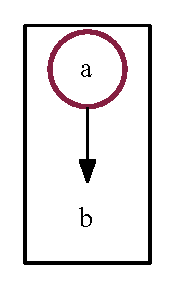
\includegraphics[scale=0.6666]{../graphics/initial-complete.pdf} &
			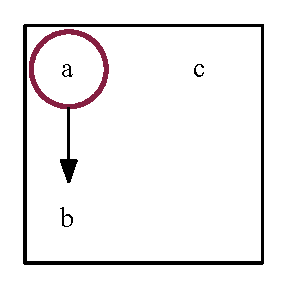
\includegraphics[scale=0.6666]{../graphics/initial-incomplete.pdf} &
			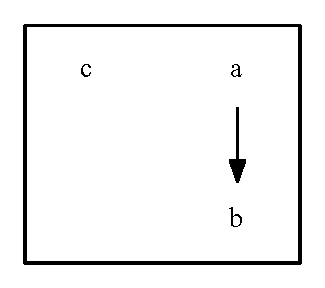
\includegraphics[scale=0.6666]{../graphics/no-initial-incomplete.pdf}\\
			(a) & (b) & (c)
		\end{tabular}
		\caption{Three graphical representations of local stemmata with and without an initial text reading; the initial text, if it has been decided, is circled in maroon. (a) A complete local stemma whose root is the initial text reading. (b) An incomplete local stemma whose initial text reading is known. (c) An incomplete local stemma whose initial text reading is not known. The scenario of a complete local stemma whose initial text is not known is excluded because if the local stemma is complete, then by definition, it will have a reading that has paths to all other readings in the stemma, and this in turn must be the reading of the initial text.}
		\label{fig:initial-text}
	\end{figure}
	
	A few comments are in order. The initial text, like the local stemmata, is an \emph{input} to the CBGM, reflecting the textual critic's preliminary judgment of intrinsic factors of variant readings, as opposed to an \emph{output} of the CBGM. The CBGM is not designed to extrapolate the earliest form of the text from scratch; the textual critic is expected to provided as complete a picture of the initial text as possible up front. The CBGM can then use the complete parts of the picture (in terms of the known readings of \emph{A} and known relationships in local stemmata) to help its users fill in the incomplete parts. (See Section \ref{sec:textual-flow} for an illustration of how this is done.) In this way, the CBGM supports the refinement of hypotheses about the initial text.
	
	\newpage
	
	\subsection{Pre-genealogical and Genealogical Relationships}\label{subsec:relationships}
	Since witnesses are sets of variant readings in the CBGM, their relationships can be inferred from relationships between their corresponding readings. The CBGM distinguishes between two types of relationships between readings: \emph{pre-genealogical}, which concerns simple agreement and disagreement, and \emph{genealogical}, which accounts for directional relationships between readings as defined in local stemmata. The genealogical relationship of reading \emph{a} relative to reading \emph{b} can be broken down into the following cases:
	\begin{itemize}
		\item\emph{agreement}: Readings \emph{a} and \emph{b} are the same. If subvariants, split attestations, ambiguities, etc. are merged with their parent readings, then they are counted as agreeing with those readings. Two lacunae are \emph{not} counted as agreeing.
		\item\emph{priority}: There is a path starting at \emph{a} and ending at \emph{b} in the local stemma.
		\item\emph{posteriority}: Reading \emph{b} is prior to reading \emph{a}.
		\item\emph{no relationship}: There is a reading prior to both \emph{a} and \emph{b}, but neither of \emph{a} and \emph{b} is prior to the other.
		\item\emph{unclear relationship}: Readings \emph{a} and \emph{b} have no common reading prior to both of them. This only happens when the local stemma is incomplete.
	\end{itemize}
	These cases are illustrated in Fig.~\ref{fig:genealogical-relationships}.
	
	\begin{figure}[h!]
		\centering
		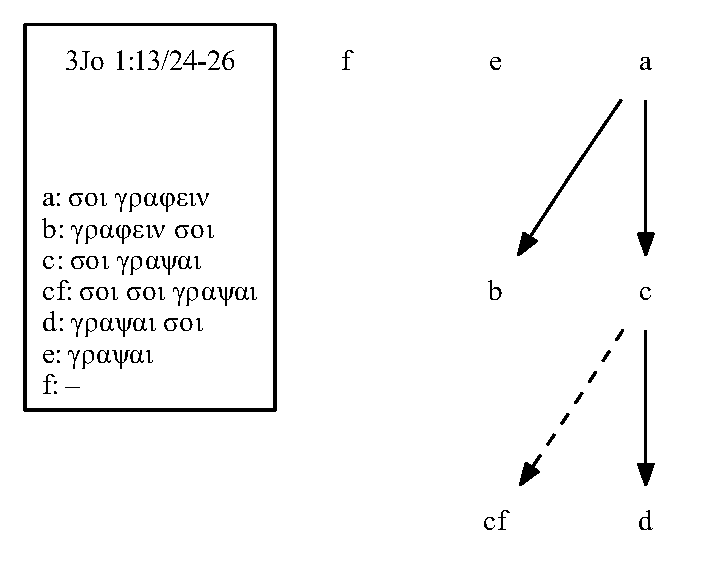
\includegraphics[scale=0.6666]{../graphics/B25K1V13U24-26-local-stemma.pdf}
		\caption{Local stemma of 3~John 1:13\ForwardSlash 24–26. Reading \emph{c} trivially agrees with itself, and if the defective subvariant \emph{cf} is merged with \emph{c}, then the two readings agree. Reading \emph{c} is prior to reading \emph{d} and posterior to reading \emph{a}. It is known to have no relationship to reading \emph{b} (as both have developed independently from reading \emph{a}), and its relationship to readings \emph{e} and \emph{f} is unclear.}
		\label{fig:genealogical-relationships}
	\end{figure}
	
	\newpage
	
	The pre-genealogical similarity of a witness \emph{X} to another witness \emph{Y} is measured in terms of the number of passages where their readings agree. (If a proportion of agreement is desired, then the number of agreements should be divided by the number of passages where both \emph{X} and \emph{Y} are extant.) If other witnesses are sorted according to their similarity to one witness, we can find that witness's closest neighbors, as Fig.~\ref{fig:compare-witnesses} depicts.
	
	\begin{figure}[h!]
		\centering
		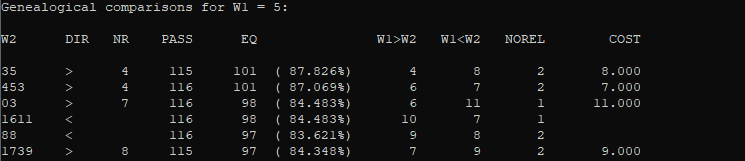
\includegraphics[width=\textwidth]{../graphics/compare-witnesses.png}
		\caption{Table listing selected other witnesses relative to GA 5, sorted by number of agreements (the \textsf{EQ} column). The \textsf{DIR} column describes the genealogical relationship of that row's witness relative to 5, and the \textsf{W1>W2} and \textsf{W1<W2} columns contain the prior and posterior reading counts that determine this relationship.}
		\label{fig:compare-witnesses}
	\end{figure}
	
	\newpage
	
	The genealogical relationship between two witnesses is likewise determined by the predominant relationship of their corresponding readings. If \emph{X} has readings prior to those of \emph{Y} more often than \emph{Y} has readings prior to those of \emph{X}, then we say that \emph{X} is prior to \emph{Y}; passages where \emph{X} and \emph{Y} agree, have no relationship, or have an unclear relationship are not counted. From the perspective of the the CBGM, this means that witness \emph{X} is a \emph{potential ancestor} of \emph{Y} in a reconstruction of the text's history. Thus defined, potential ancestry induces a convenient ordering on witnesses, as Fig.~\ref{fig:potential-ancestors} shows. This ordering facilitates the construction of the more complex elements of the CBGM to which we now turn.
	
	\begin{figure}[h!]
		\centering
		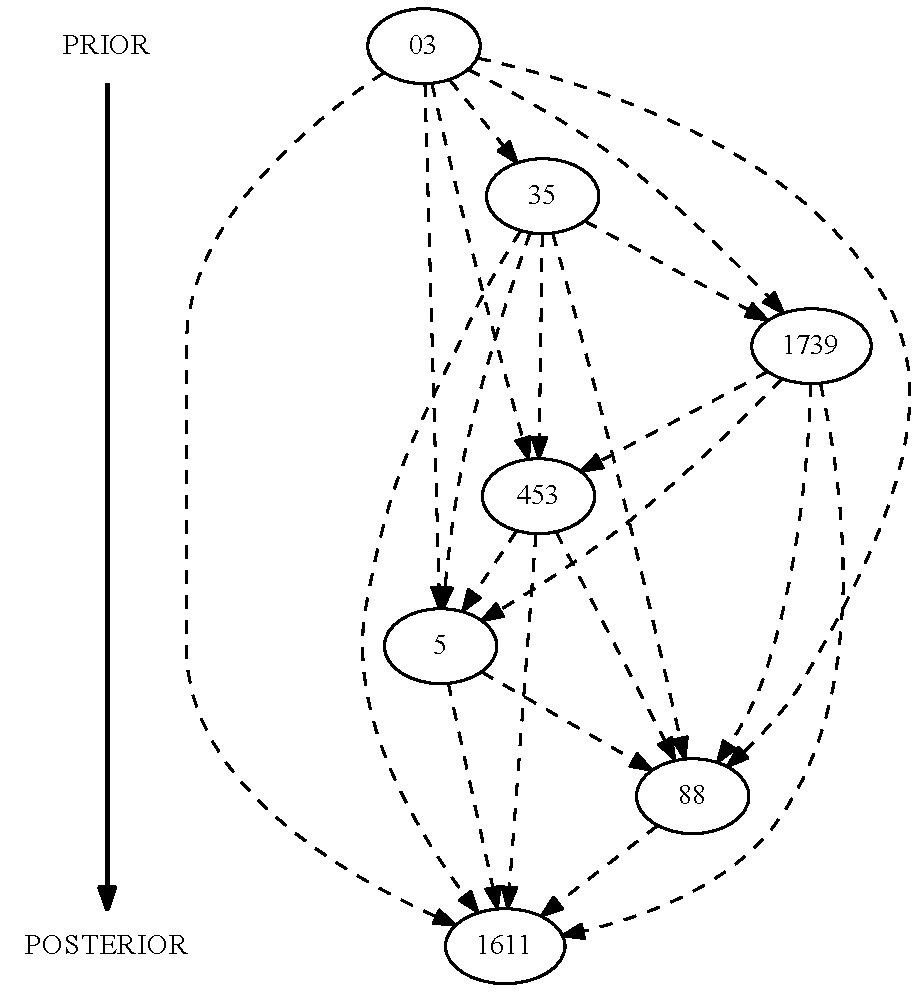
\includegraphics[scale=0.6666]{../graphics/potential-ancestors.pdf}
		\caption{Graph of potential ancestry relationships between the witnesses compared in Fig.~\ref{fig:compare-witnesses}. The lines are dashed to indicate that these relationships are only tentative; the most likely ancestry relationships in the reconstruction of textual history are determined at a later stage.}
		\label{fig:potential-ancestors}
	\end{figure}
	
	\newpage
	
	\section{Textual Flow}\label{sec:textual-flow}
	A \emph{textual flow diagram} is a graph that uses witnesses' pre-genealogical and genealogical relationships throughout a text to identify their most likely sources for a reading in a specific passage. Textual flow diagrams organize witnesses in way that facilitates validation and revision of local stemmata and hypotheses about the initial text.
	
	In a textual flow diagram, each witness is assigned a single textual flow ancestor from its set of potential ancestors. The only witnesses without textual flow ancestors are those without any potential ancestors, such as the initial text \emph{A} and any fragmentary witnesses that agree with \emph{A} in all of their extant passages. In the interest of parsimony (i.e., assuming as few changed readings as possible), a witness's textual flow ancestor should have high pre-genealogical similarity to it, and it should share its reading in the passage under consideration. To balance these considerations, a \emph{connectivity limit} κ associated with the textual flow diagram can narrow a witness's pool of textual flow ancestors to its κ closest potential ancestors (see Fig.~\ref{fig:find-relatives}).
	
	\begin{figure}[h!]
		\centering
		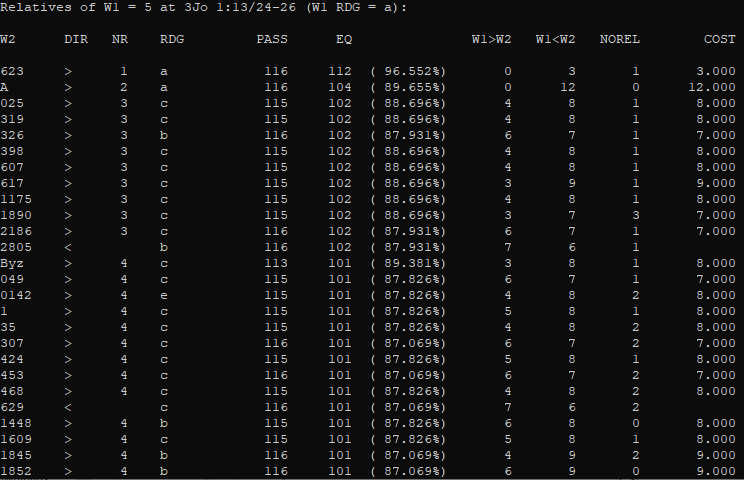
\includegraphics[width=\textwidth]{../graphics/find-relatives.png}
		\caption{Table of relatives for GA 5 in 3~John 1:13\ForwardSlash 24–26. The \textsf{NR} column lists the ranks of 5's potential ancestors, determined by their number of agreements with 5 throughout the text of 3~John. (Potential ancestors with the same number of agreements are assigned the same rank; non-ancestors are not assigned any rank.) Since 5 has reading \emph{a} in this passage, GA 623 is its textual flow ancestor. If it had reading \emph{b} and the connectivity limit κ was at least 3, then GA 326 would be its ancestor.}
		\label{fig:find-relatives}
	\end{figure}
	
	\newpage
	
	\subsection{Construction}
	
	The process of selecting the textual flow ancestor of a given witness \emph{X} at a given passage with a connectivity limit κ consists of the following steps:
	\begin{enumerate}
		\item Sort the potential ancestors of \emph{X} in descending order of their pre-genealogical similarity to \emph{X}.
		\item Filter out any potential ancestors whose ancestral rank (see Fig.~\ref{fig:find-relatives} for details) is greater than κ.
		\item If any of the remaining potential ancestors shares the reading of \emph{X} in this passage, then the choose the first one that does; otherwise, choose the first potential ancestor that is not lacunose in this passage.
	\end{enumerate}
	The finer details of this process (how ancestral ranks should be assigned, whether witnesses that are lacunose in this passage should have textual flow ancestors, and even which potential ancestor should be chosen in step 3 if none shares the reading of \emph{X}) vary between software implementations,\footnote{The INTF's ``Genealogical Queries'' module for the \emph{Editio Critica Maior} (ECM) of the Catholic Epistles (\url{http://intf.uni-muenster.de/cbgm2/GenQ.html}), the CCeH module for the \emph{ECM} of Acts (\url{https://ntg.cceh.uni-koeln.de/acts/ph4/}), Andrew Edmondson's implementation for his dissertation on the CBGM \parencite[code available online at \url{https://github.com/edmondac/CBGM} {[DOI \href{http://doi.org/10.5281/zenodo.1296288}{10.5281/zenodo.1296288}]}]{Edmondson19}, and the \textsf{open-cbgm} library (\url{https://github.com/jjmccollum/open-cbgm}) all implement these rules slightly differently.} but the resulting textual flow diagrams typically look similar. An example diagram is shown in Fig.~\ref{fig:textual-flow}.
	
	\begin{sidewaysfigure}
		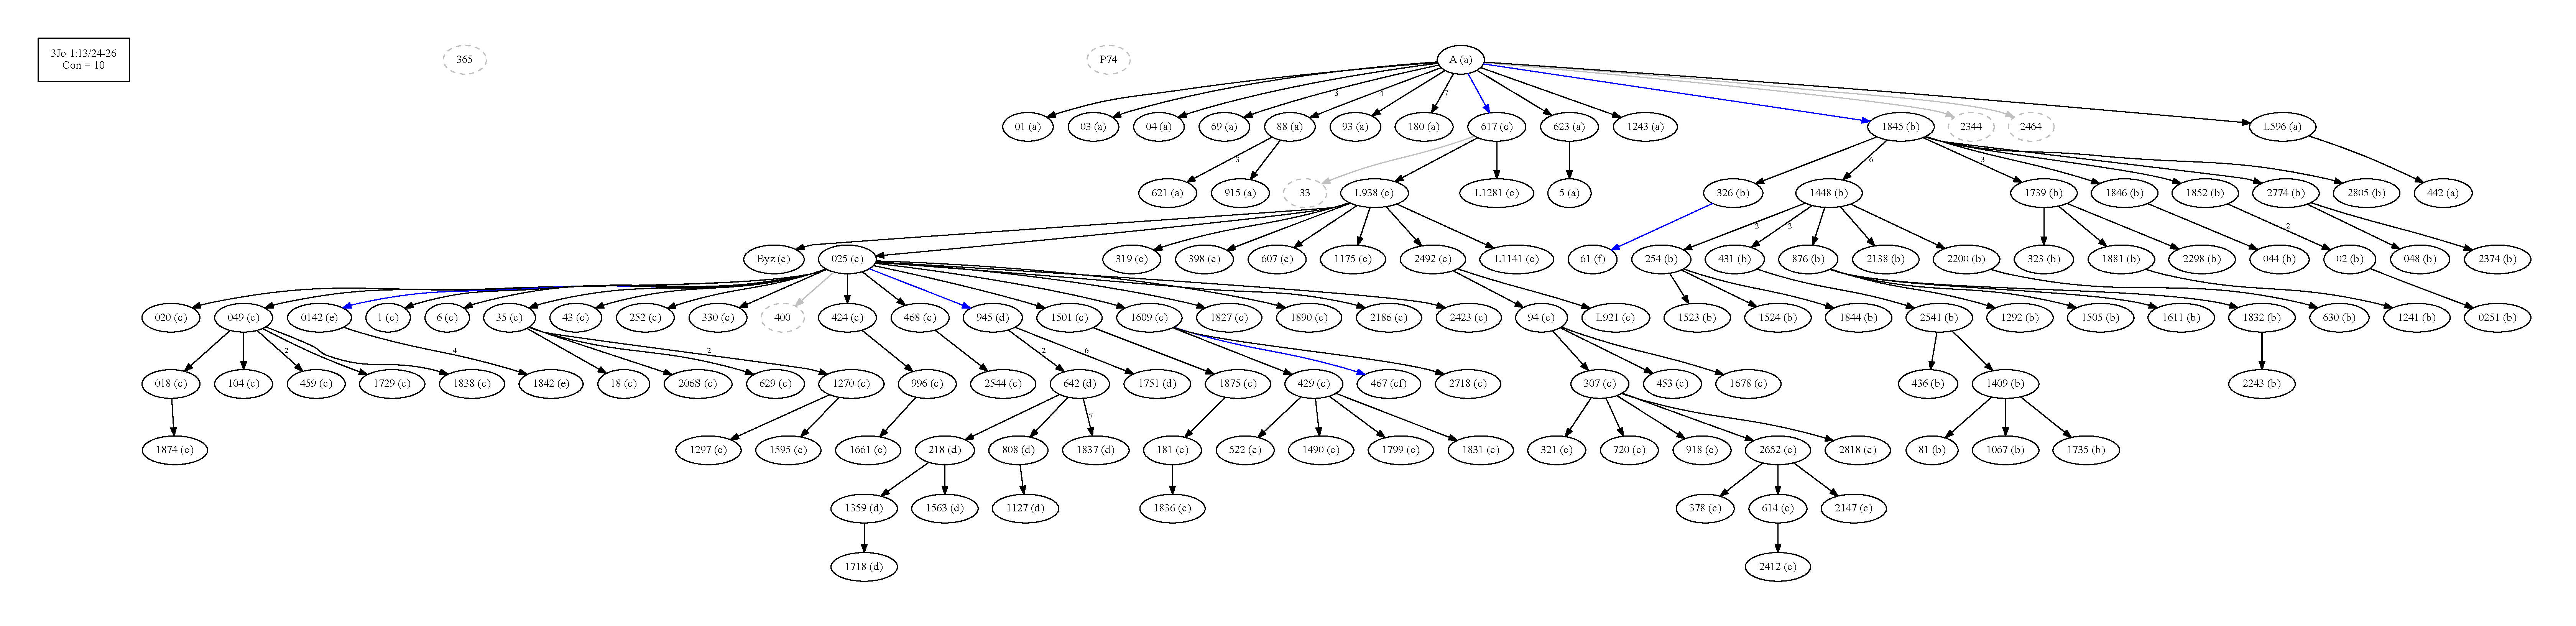
\includegraphics[width=\textwidth]{../graphics/B25K1V13U24-26-textual-flow.pdf}
		\caption{Complete textual flow diagram for 3~John 1:13\ForwardSlash 24–26 with a connectivity limit of κ=10. Witnesses are listed alongside their readings in this passage. Witnesses with dotted outlines are lacunose in this passage. While textual flow proceeds from the initial text \emph{A} to most witnesses, two witnesses (GA \Pap{74} and 365) are too fragmentary for their potential ancestors to be inferred. Black lines represent textual flow in which the reading of the textual flow ancestor is preserved by the textual flow descendant. Blue lines represent textual flow in which a change is introduced. Gray lines represent textual flow to lacunose witnesses.}
		\label{fig:textual-flow}
	\end{sidewaysfigure}
	
	\newpage
	
	\subsection{Revising the Initial Text}\label{subsec:revising-initial-text}
	As we mentioned in Subsection \ref{subsec:initial-text}, the CBGM offers textual critics a way to refine their hypotheses about the readings of the initial text \emph{A}. While the complete textual flow diagram that includes all witnesses can be used to this end, it is more practical to use a smaller graph, the \emph{coherence in attestations diagram}, that focuses on witnesses that support a specific reading in a passage. By way of example, let us continue with 3~John 1:13\ForwardSlash 24–26.
	
	While the editors of the \emph{Editio Critica Maior} (ECM) judged reading \emph{a} (σοι γραφειν) to be the initial reading, the transposition γραφειν σοι of reading \emph{b} has early and reasonably widespread support, and the substitution σοι γραψαι of reading \emph{c} has the support of many Byzantine and non-Byzantine witnesses. We could compare the hypothesis of reading \emph{a}'s priority to alternative hypotheses in which the initial text reads \emph{b} or \emph{c}. The primary metric for this comparison is \emph{coherence}, traditionally quantified as the number of independent origins of a given reading. As Figs.~\ref{fig:coherence-a-1}, \ref{fig:coherence-b-1}, and \ref{fig:coherence-c-1} demonstrate, each reading has only one point of origin when \emph{a} is assumed to be the initial reading, which constitutes perfect coherence. The parsimony with which each reading can be explained supports the hypothesis that \emph{a} is the earliest reading.
	
	\begin{sidewaysfigure}
		\centering
		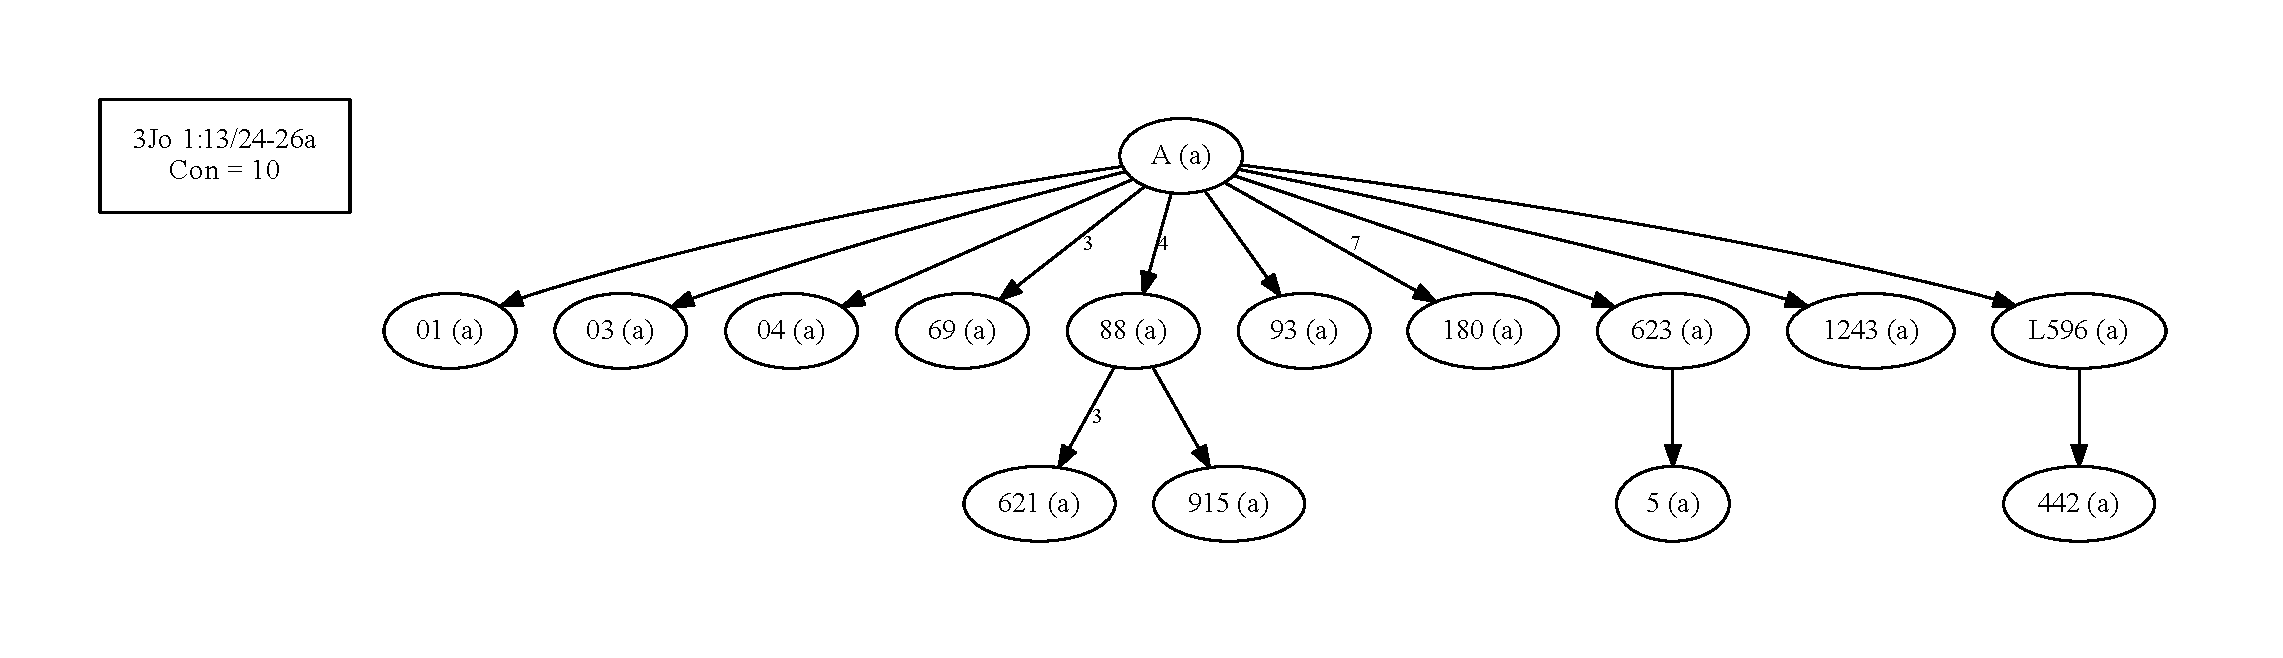
\includegraphics[scale=0.3333]{../graphics/B25K1V13U24-26Ra-coherence-attestations-1.pdf}
		\caption{Coherence in attestations diagram for 3~John 1:13\ForwardSlash 24–26, reading \emph{a}, with \emph{a} assumed to be the initial reading.}
		\label{fig:coherence-a-1}
	\end{sidewaysfigure}
	
	\begin{sidewaysfigure}
		\centering
		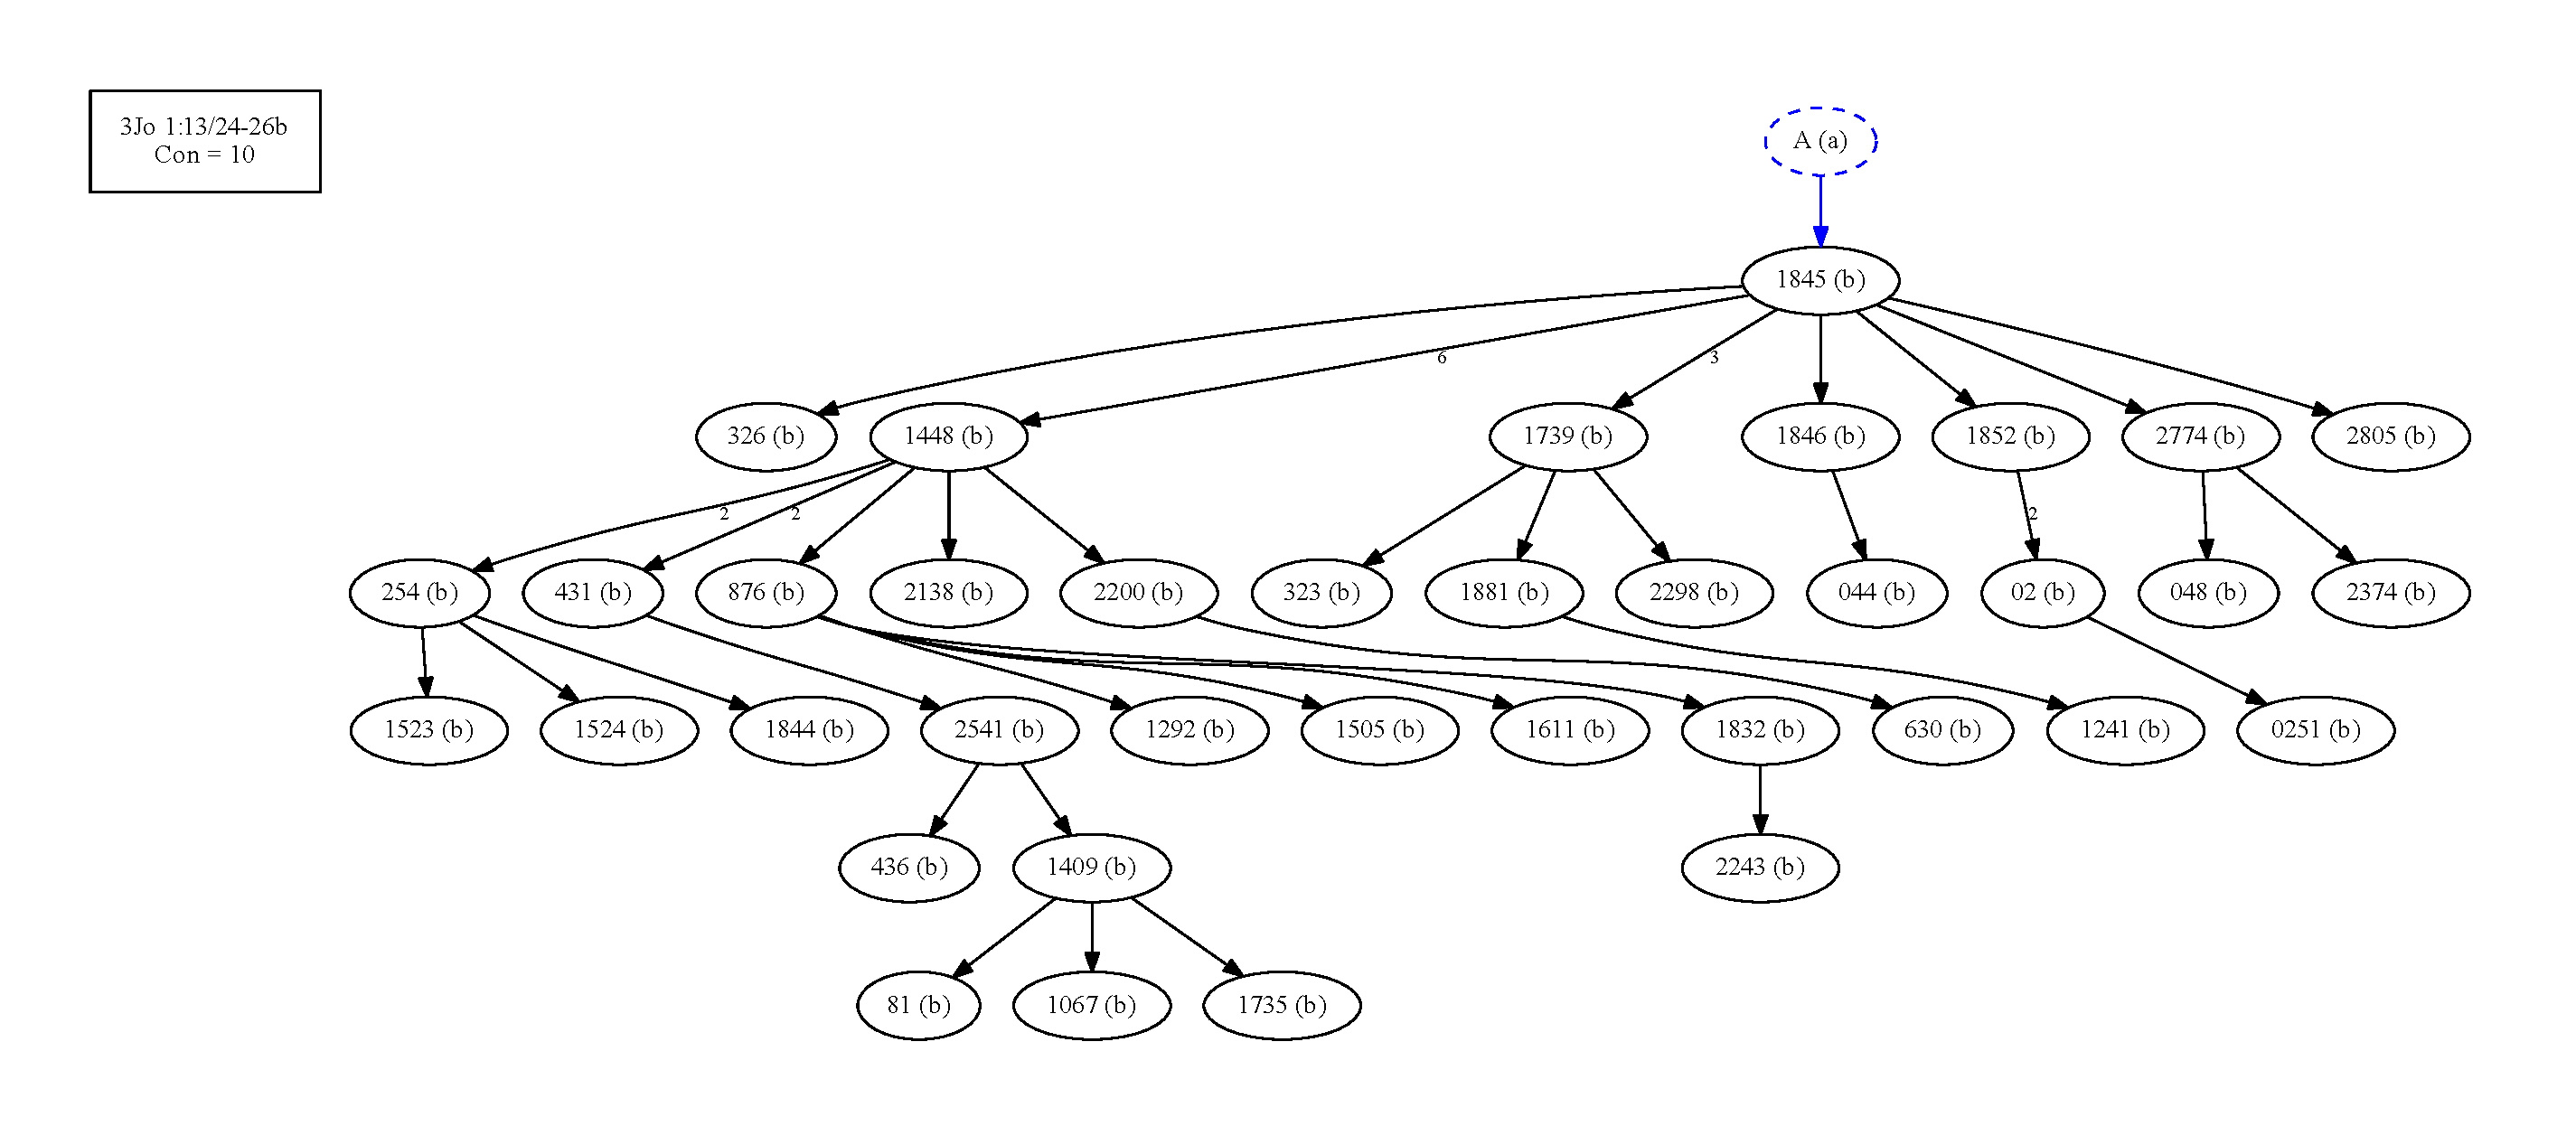
\includegraphics[scale=0.3333]{../graphics/B25K1V13U24-26Rb-coherence-attestations-1.pdf}
		\caption{Coherence in attestations diagram for 3~John 1:13\ForwardSlash 24–26, reading \emph{b}, with \emph{a} assumed to be the initial reading.}
		\label{fig:coherence-b-1}
	\end{sidewaysfigure}
	
	\begin{sidewaysfigure}
		\centering
		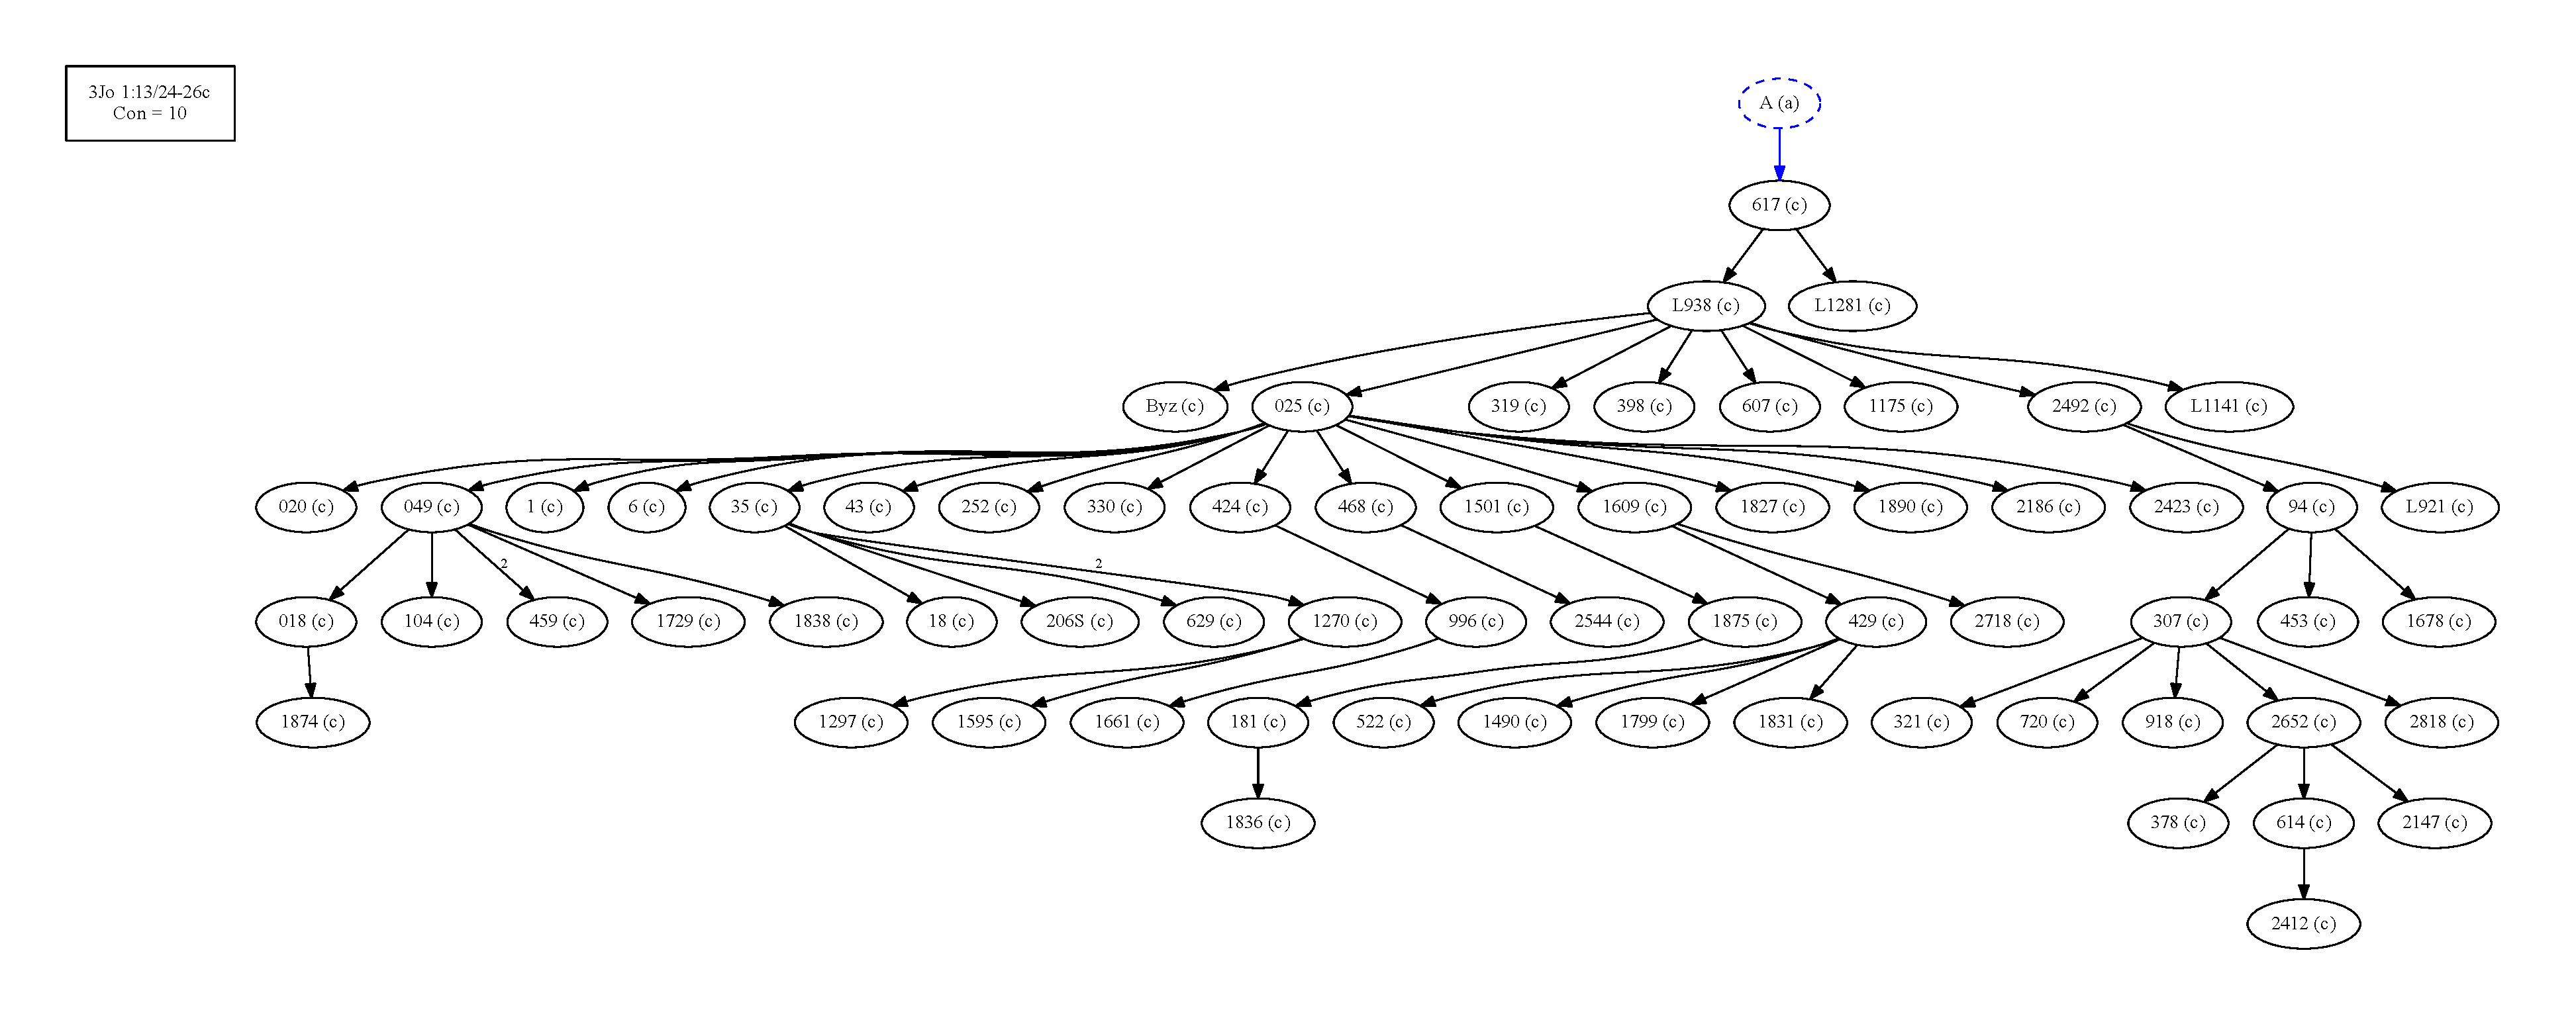
\includegraphics[scale=0.3333]{../graphics/B25K1V13U24-26Rc-coherence-attestations-1.pdf}
		\caption{Coherence in attestations diagram for 3~John 1:13\ForwardSlash 24–26, reading \emph{c}, with \emph{a} assumed to be the initial reading.}
		\label{fig:coherence-c-1}
	\end{sidewaysfigure}
	
	\newpage
	
	If we wanted to evaluate the hypothesis that reading \emph{b} was the initial reading, then we would assign the support of the initial text \emph{A} to this reading, and we would reverse the orientation of the genealogical relationship between readings \emph{a} and \emph{b} in the local stemma, as shown in Fig.~\ref{fig:local-stemma-b-initial}.
	
	\begin{figure}[h!]
		\centering
		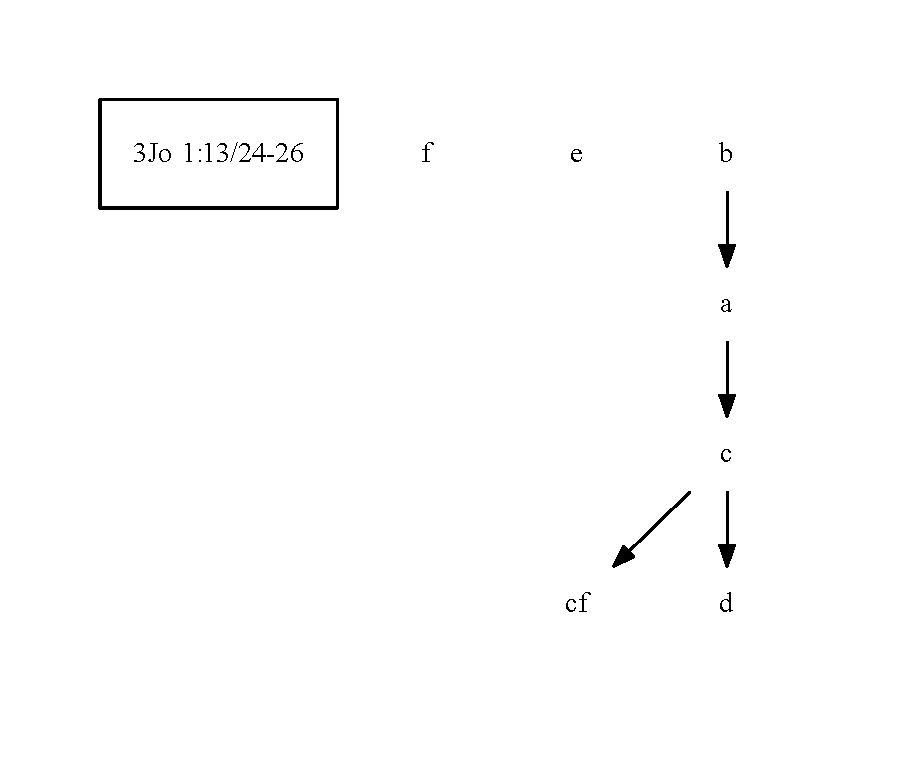
\includegraphics[scale=0.6666]{../graphics/B25K1V13U24-26-local-stemma-b-initial.pdf}
		\caption{Local stemma of 3~John 1:13\ForwardSlash 24–26, reoriented so that \emph{b} is the initial text reading.}
		\label{fig:local-stemma-b-initial}
	\end{figure}
	\noindent
	This would yield the coherence in attestations diagrams pictured in Figs.~\ref{fig:coherence-a-2}, \ref{fig:coherence-b-2}, and \ref{fig:coherence-c-2}.
	
	\begin{sidewaysfigure}
		\centering
		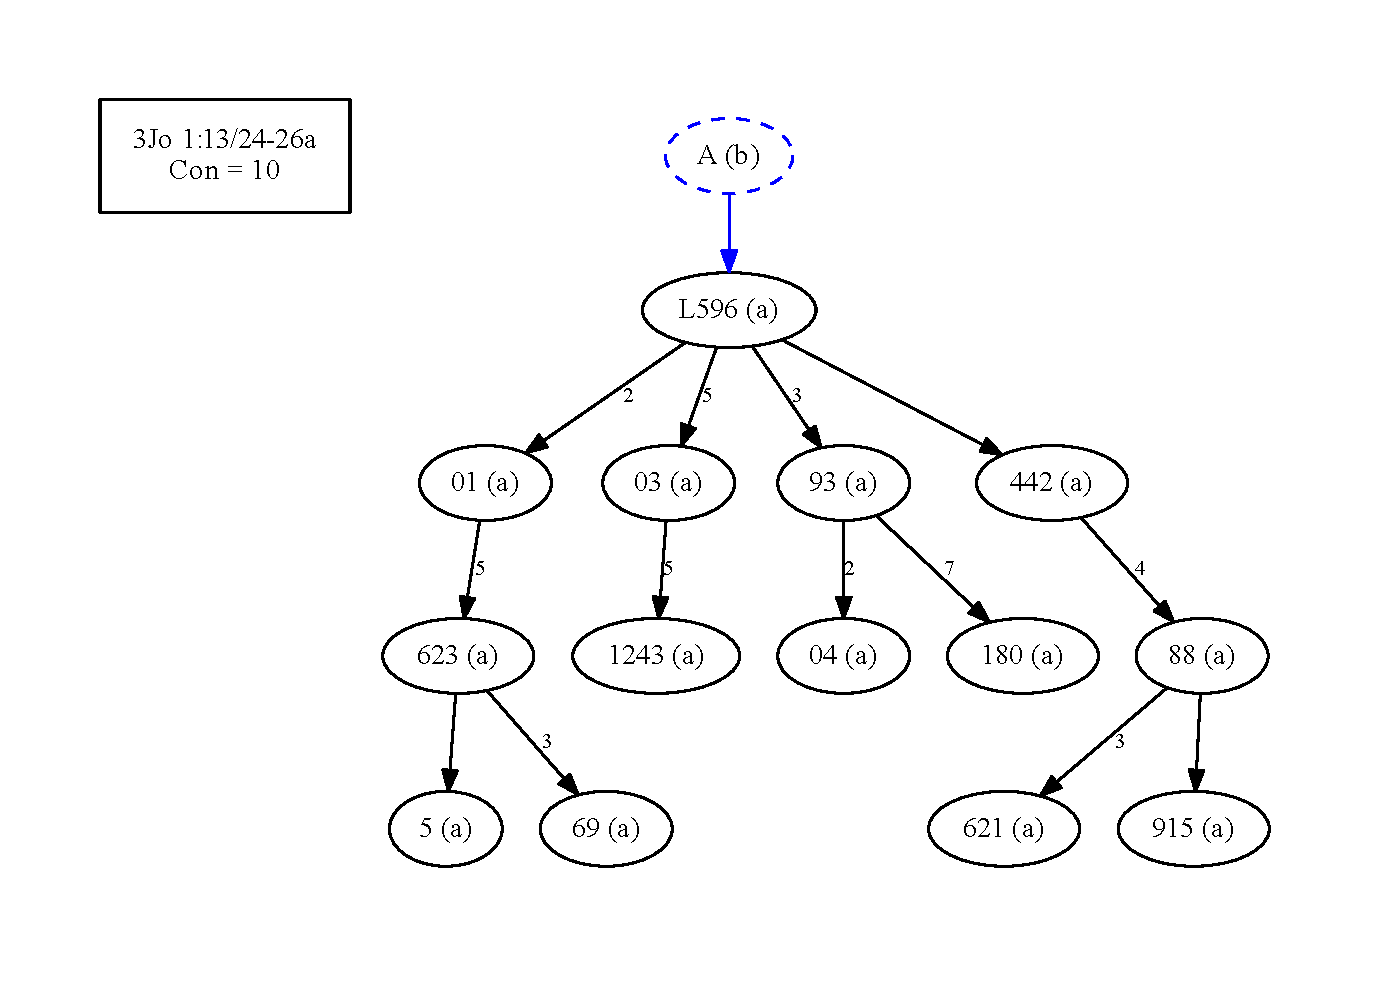
\includegraphics[scale=0.3333]{../graphics/B25K1V13U24-26Ra-coherence-attestations-2.pdf}
		\caption{Coherence in attestations diagram for 3~John 1:13\ForwardSlash 24–26, reading \emph{a}, with \emph{b} assumed to be the initial reading.}
		\label{fig:coherence-a-2}
	\end{sidewaysfigure}
	
	\begin{sidewaysfigure}
		\centering
		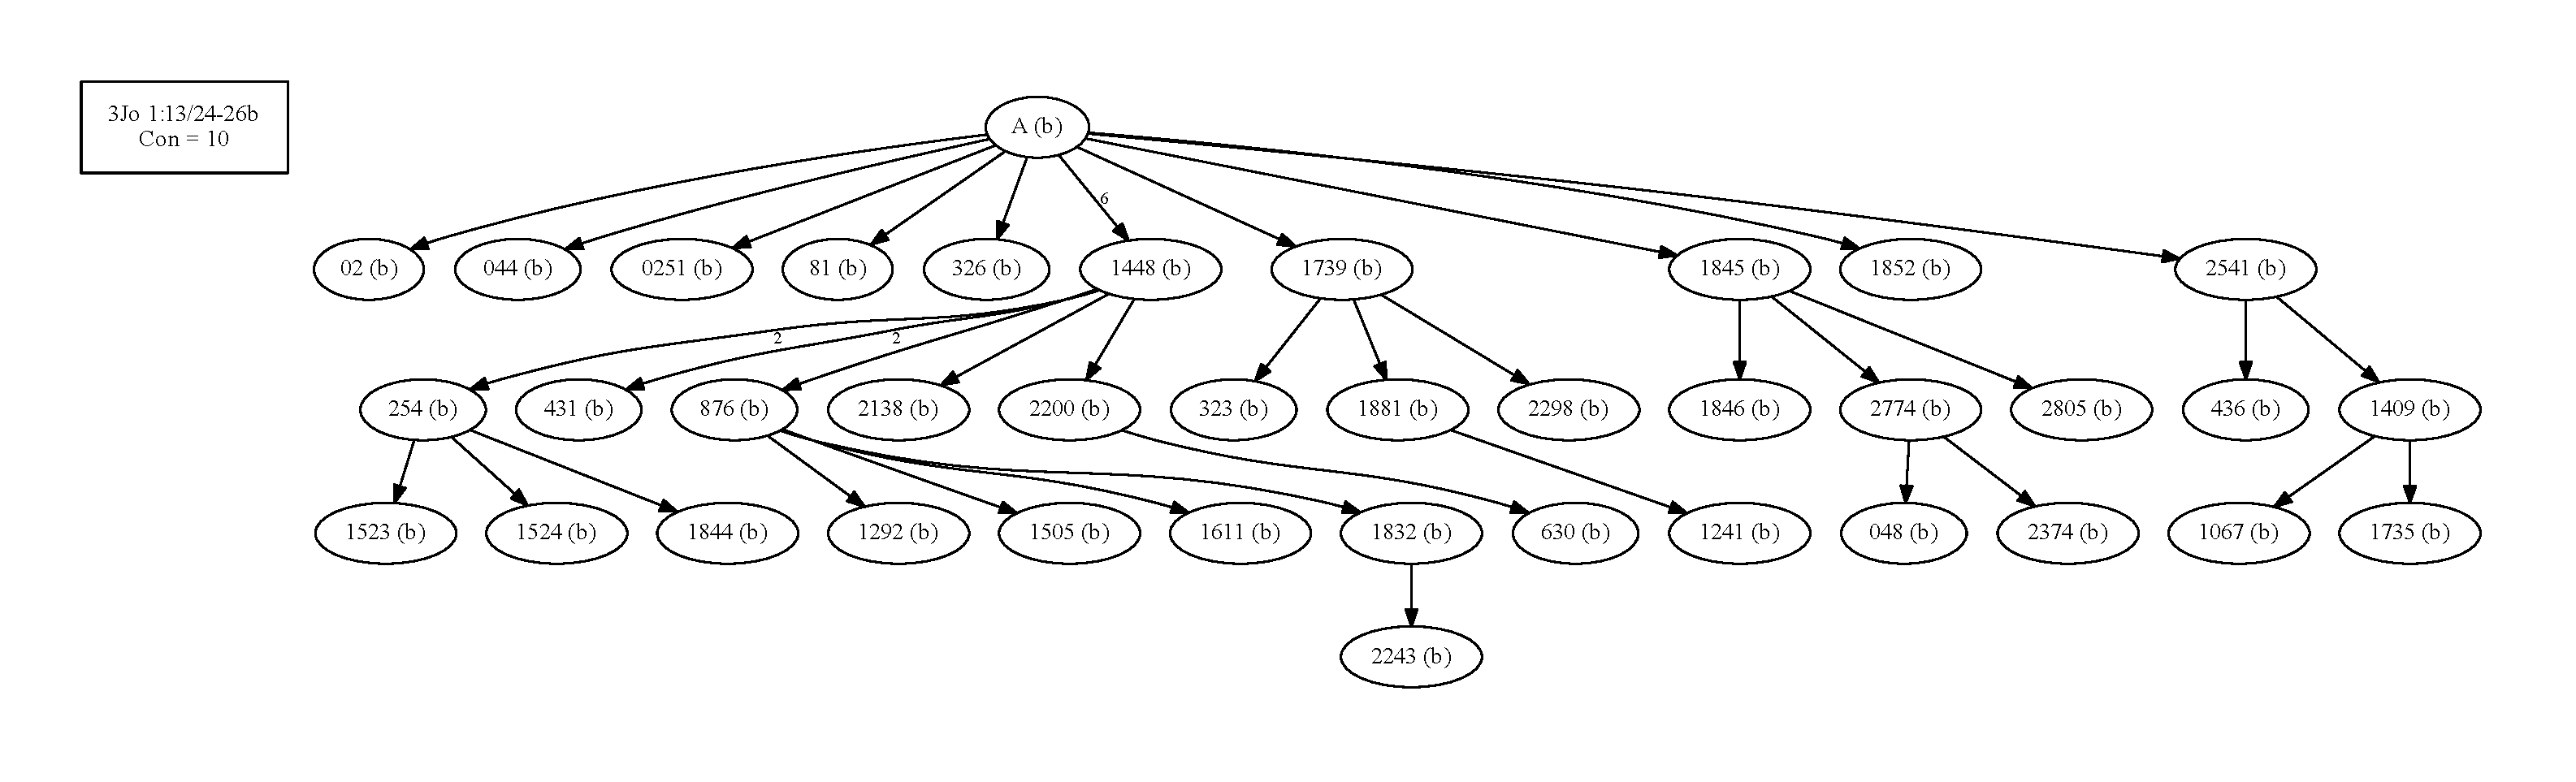
\includegraphics[scale=0.3333]{../graphics/B25K1V13U24-26Rb-coherence-attestations-2.pdf}
		\caption{Coherence in attestations diagram for 3~John 1:13\ForwardSlash 24–26, reading \emph{b}, with \emph{b} assumed to be the initial reading.}
		\label{fig:coherence-b-2}
	\end{sidewaysfigure}
	
	\begin{sidewaysfigure}
		\centering
		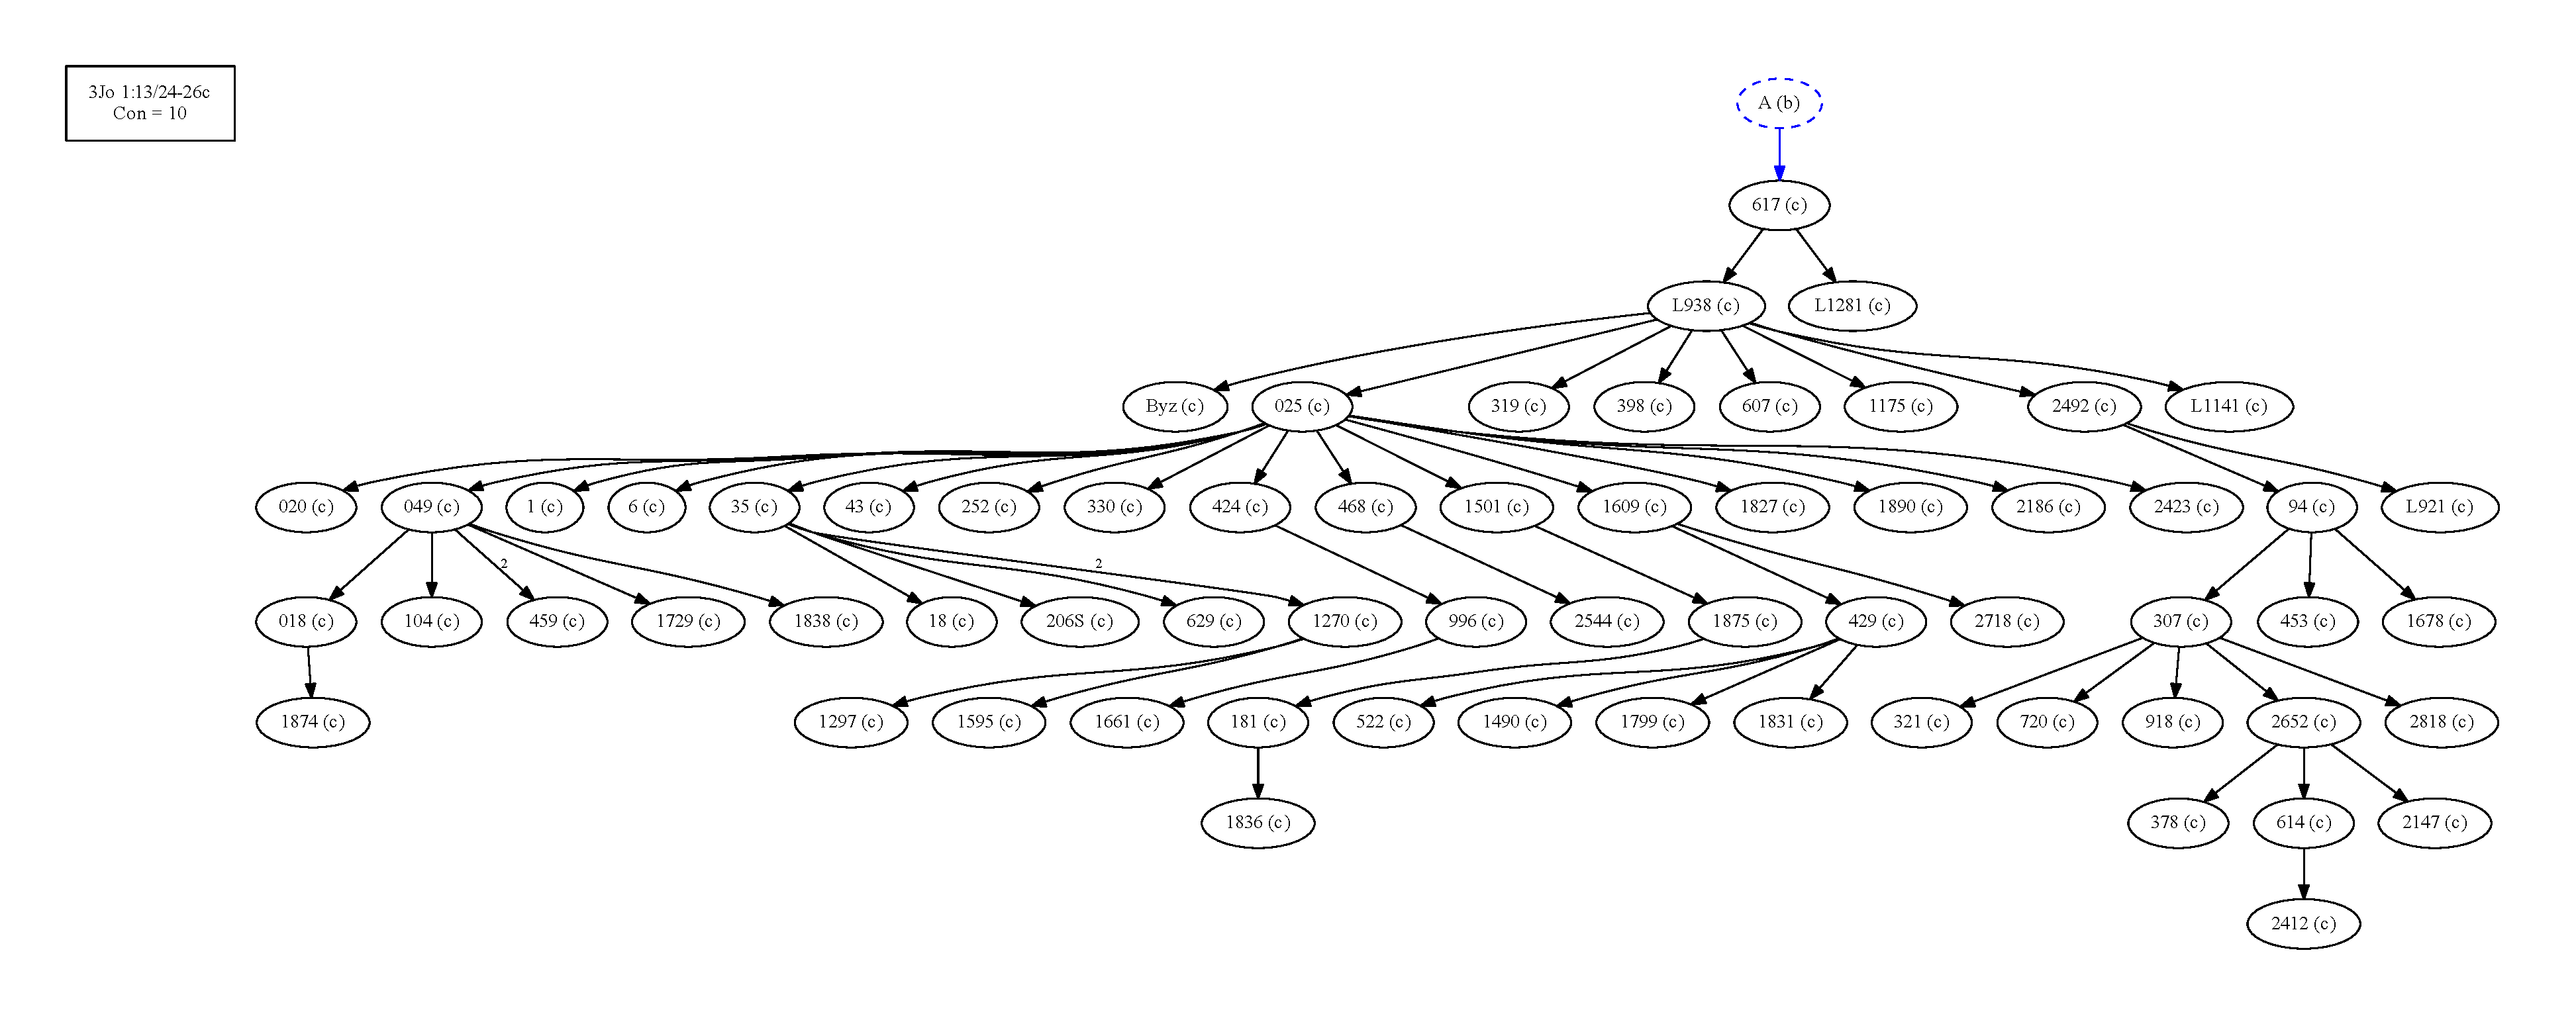
\includegraphics[scale=0.3333]{../graphics/B25K1V13U24-26Rc-coherence-attestations-2.pdf}
		\caption{Coherence in attestations diagram for 3~John 1:13\ForwardSlash 24–26, reading \emph{c}, with \emph{b} assumed to be the initial reading.}
		\label{fig:coherence-c-2}
	\end{sidewaysfigure}
	
	\newpage
	
	As we can see, all three readings still have perfect coherence. This time, however, the only emergence of reading \emph{c} is traced to a witness with reading \emph{b}, and the hypothesis represented by the local stemma of Fig.~\ref{fig:local-stemma-b-initial} does not account for any change from reading \emph{b} to reading \emph{c}.
	
	This could mean one of several things. It could mean that there is a gap in the surviving evidence where there once was a witness to reading \emph{a} between witnesses \emph{A} and GA 617. This is certainly possible, but it is also a scenario that we do not have to hypothesize if we just suppose instead that reading \emph{a} is the earliest reading. A second possibility is that the local stemma is wrong and should be revised so that reading \emph{b} gives rise to reading \emph{c} directly, but this is less plausible on internal grounds; a change from reading \emph{a} to reading \emph{c} only requires a change in verb tense, while a change from reading \emph{b} to reading \emph{c} requires a change in tense and a transposition. The last possibility is that the assumption of reading \emph{b}'s priority is problematic.
	
	To evaluate the hypothesis of priority for reading \emph{c}, then we would assign the support of the initial text \emph{A} to reading \emph{c} and reverse the orientation of the genealogical relationship between readings \emph{a} and \emph{c} in the local stemma, as shown in Fig.~\ref{fig:local-stemma-c-initial}.
	
	\begin{figure}[h!]
		\centering
		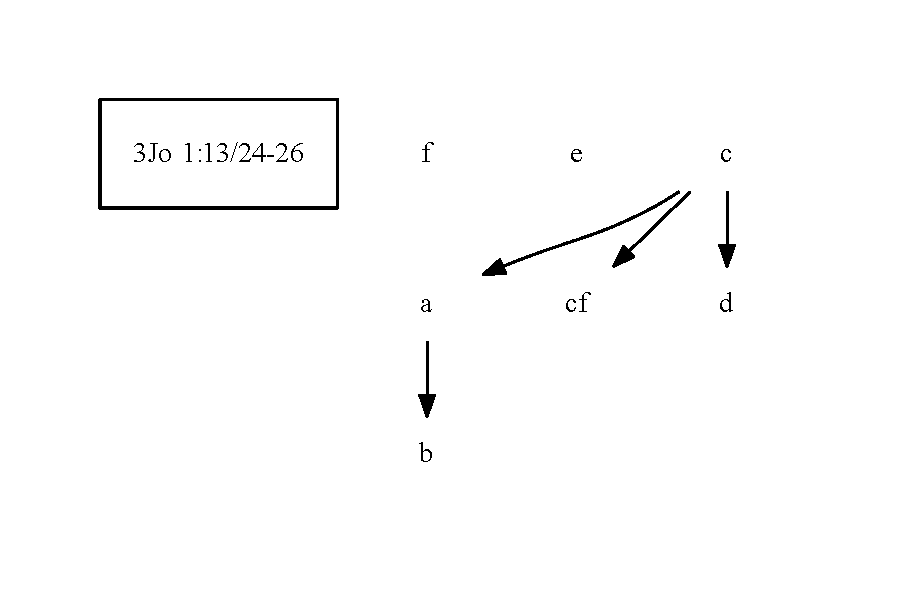
\includegraphics[scale=0.6666]{../graphics/B25K1V13U24-26-local-stemma-c-initial.pdf}
		\caption{Local stemma of 3~John 1:13\ForwardSlash 24–26, reoriented so that \emph{c} is the initial text reading.}
		\label{fig:local-stemma-c-initial}
	\end{figure}
	\noindent
	Then the coherence in attestations diagrams would appear as shown in Figs.~\ref{fig:coherence-a-3}, \ref{fig:coherence-b-3}, and \ref{fig:coherence-c-3}. In this case, all three diagrams exhibit perfect coherence and are consistent with the local stemma in Fig.~\ref{fig:local-stemma-c-initial}, so in terms of coherence, there is nothing suspicious about the hypothesis of reading \emph{c}'s primacy.
	
	\begin{sidewaysfigure}
		\centering
		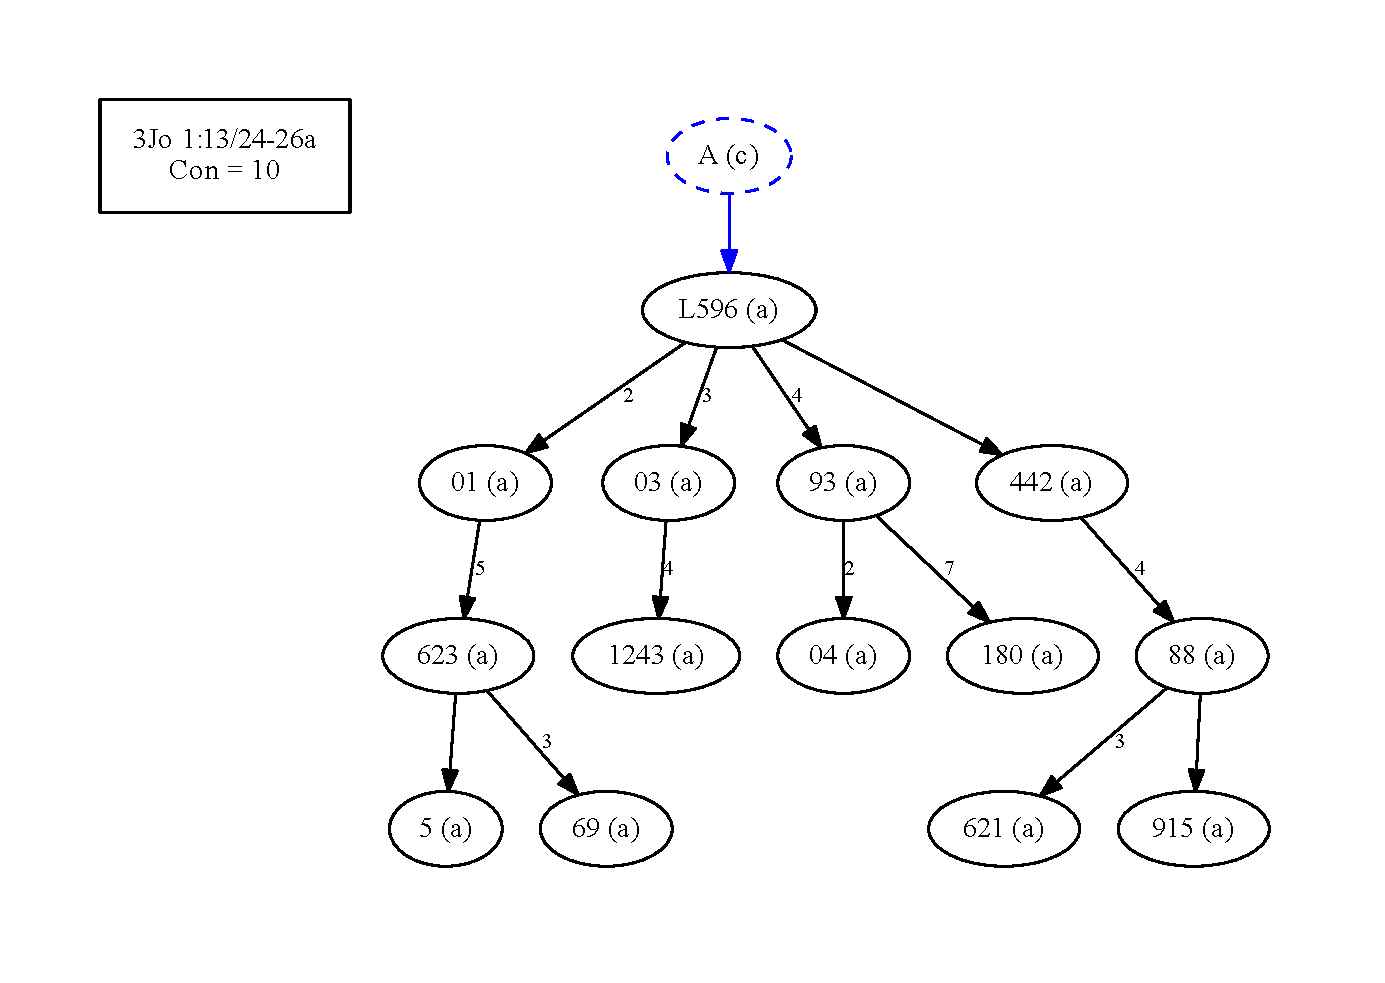
\includegraphics[scale=0.3333]{../graphics/B25K1V13U24-26Ra-coherence-attestations-3.pdf}
		\caption{Coherence in attestations diagram for 3~John 1:13\ForwardSlash 24–26, reading \emph{a}, with \emph{c} assumed to be the initial reading.}
		\label{fig:coherence-a-3}
	\end{sidewaysfigure}
	
	\begin{sidewaysfigure}
		\centering
		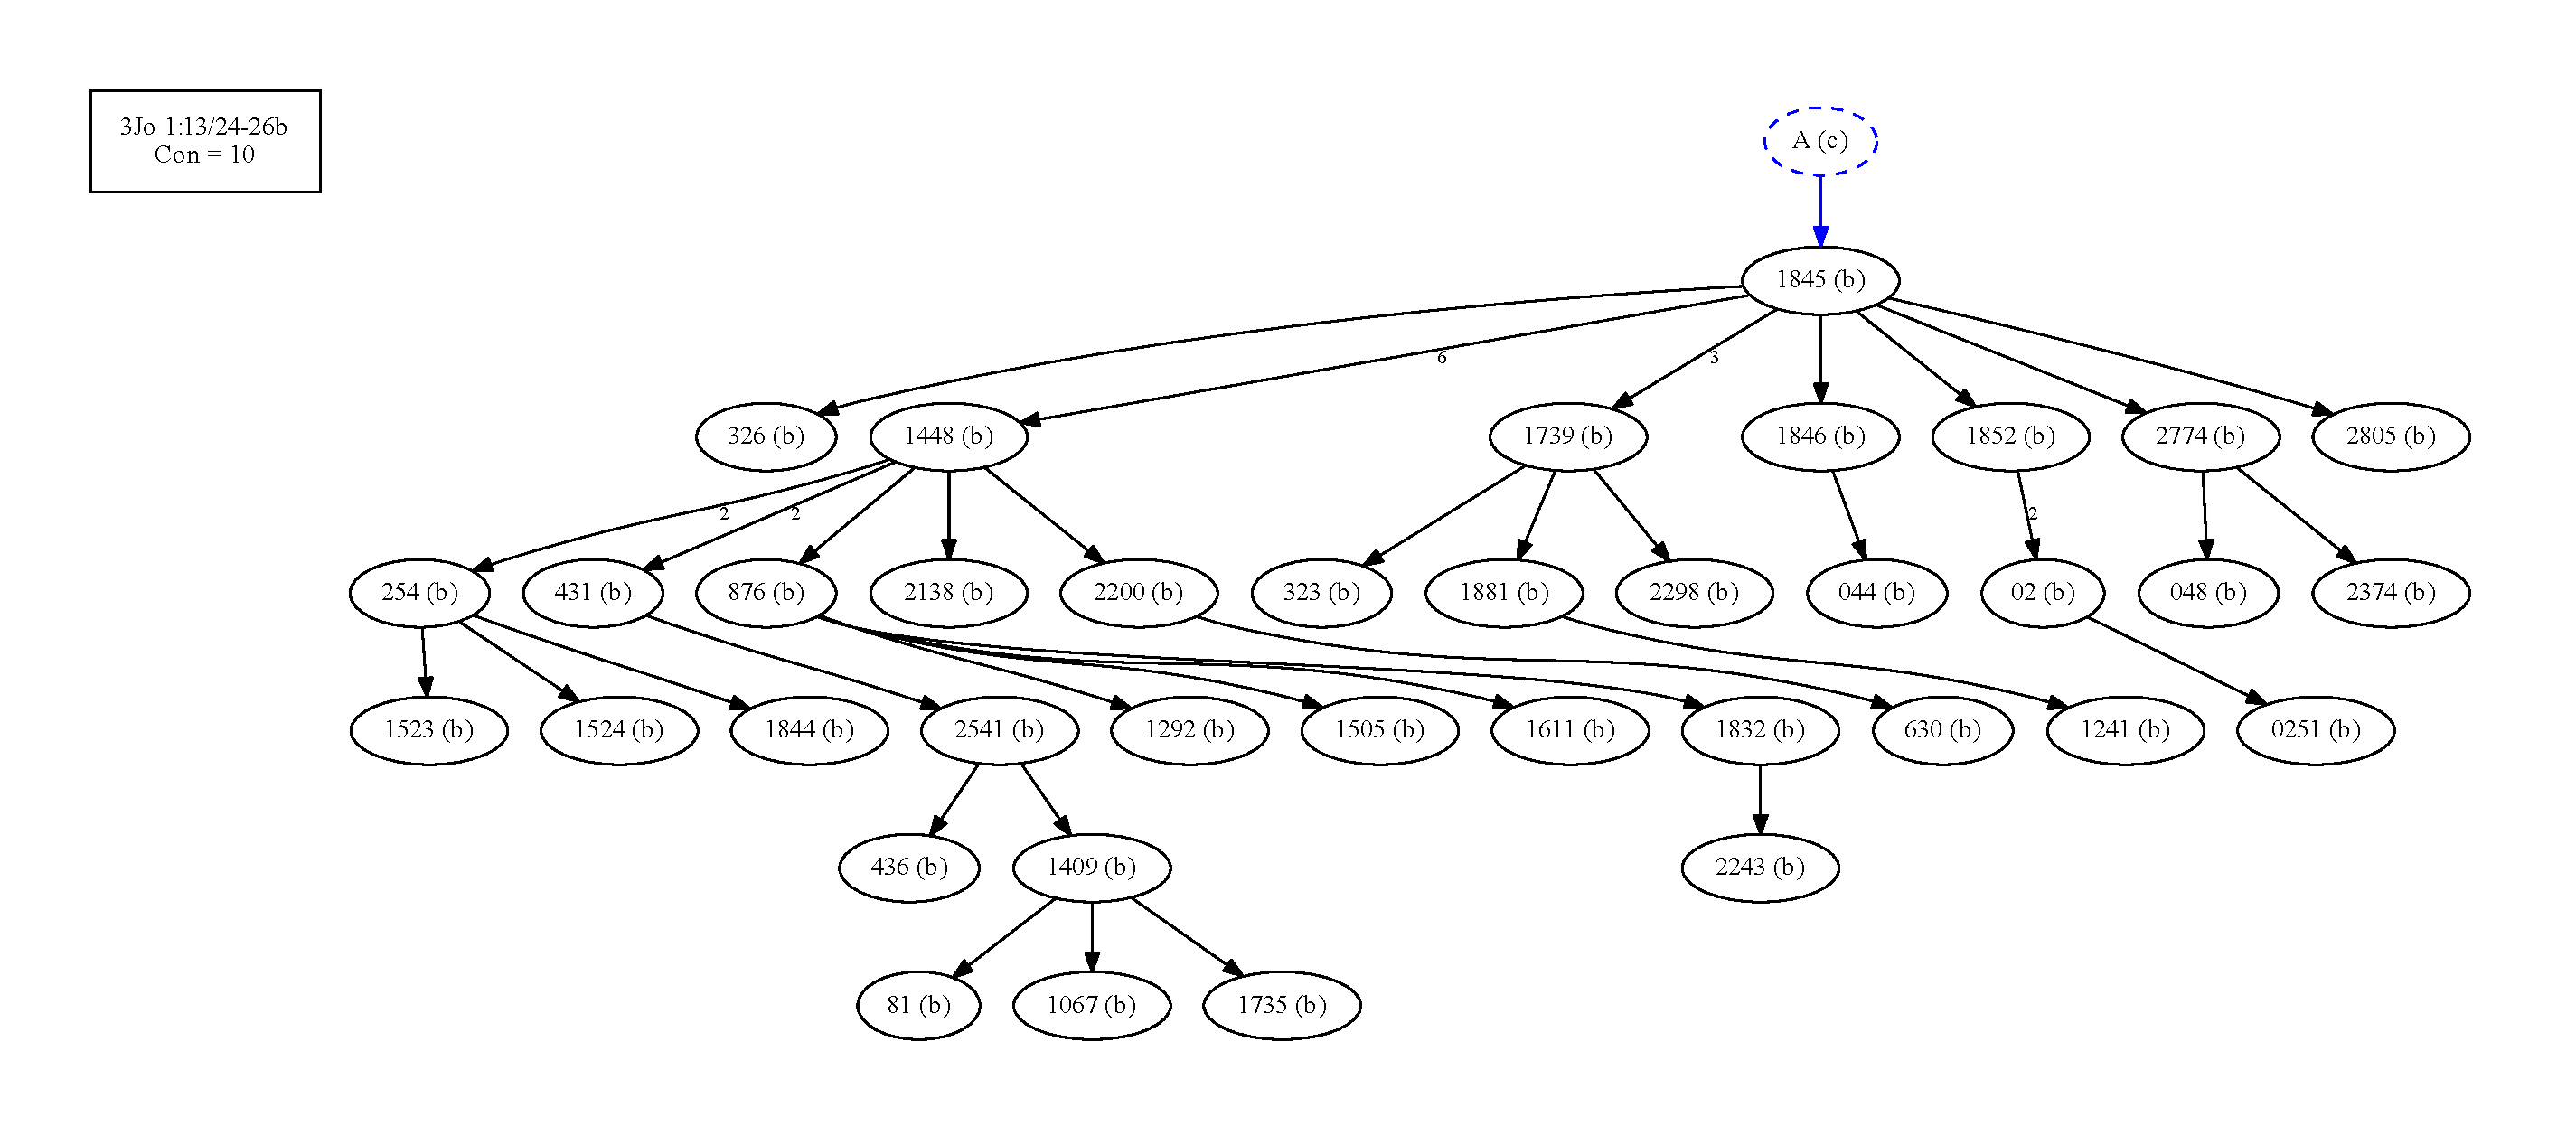
\includegraphics[scale=0.3333]{../graphics/B25K1V13U24-26Rb-coherence-attestations-3.pdf}
		\caption{Coherence in attestations diagram for 3~John 1:13\ForwardSlash 24–26, reading \emph{b}, with \emph{c} assumed to be the initial reading.}
		\label{fig:coherence-b-3}
	\end{sidewaysfigure}
	
	\begin{sidewaysfigure}
		\centering
		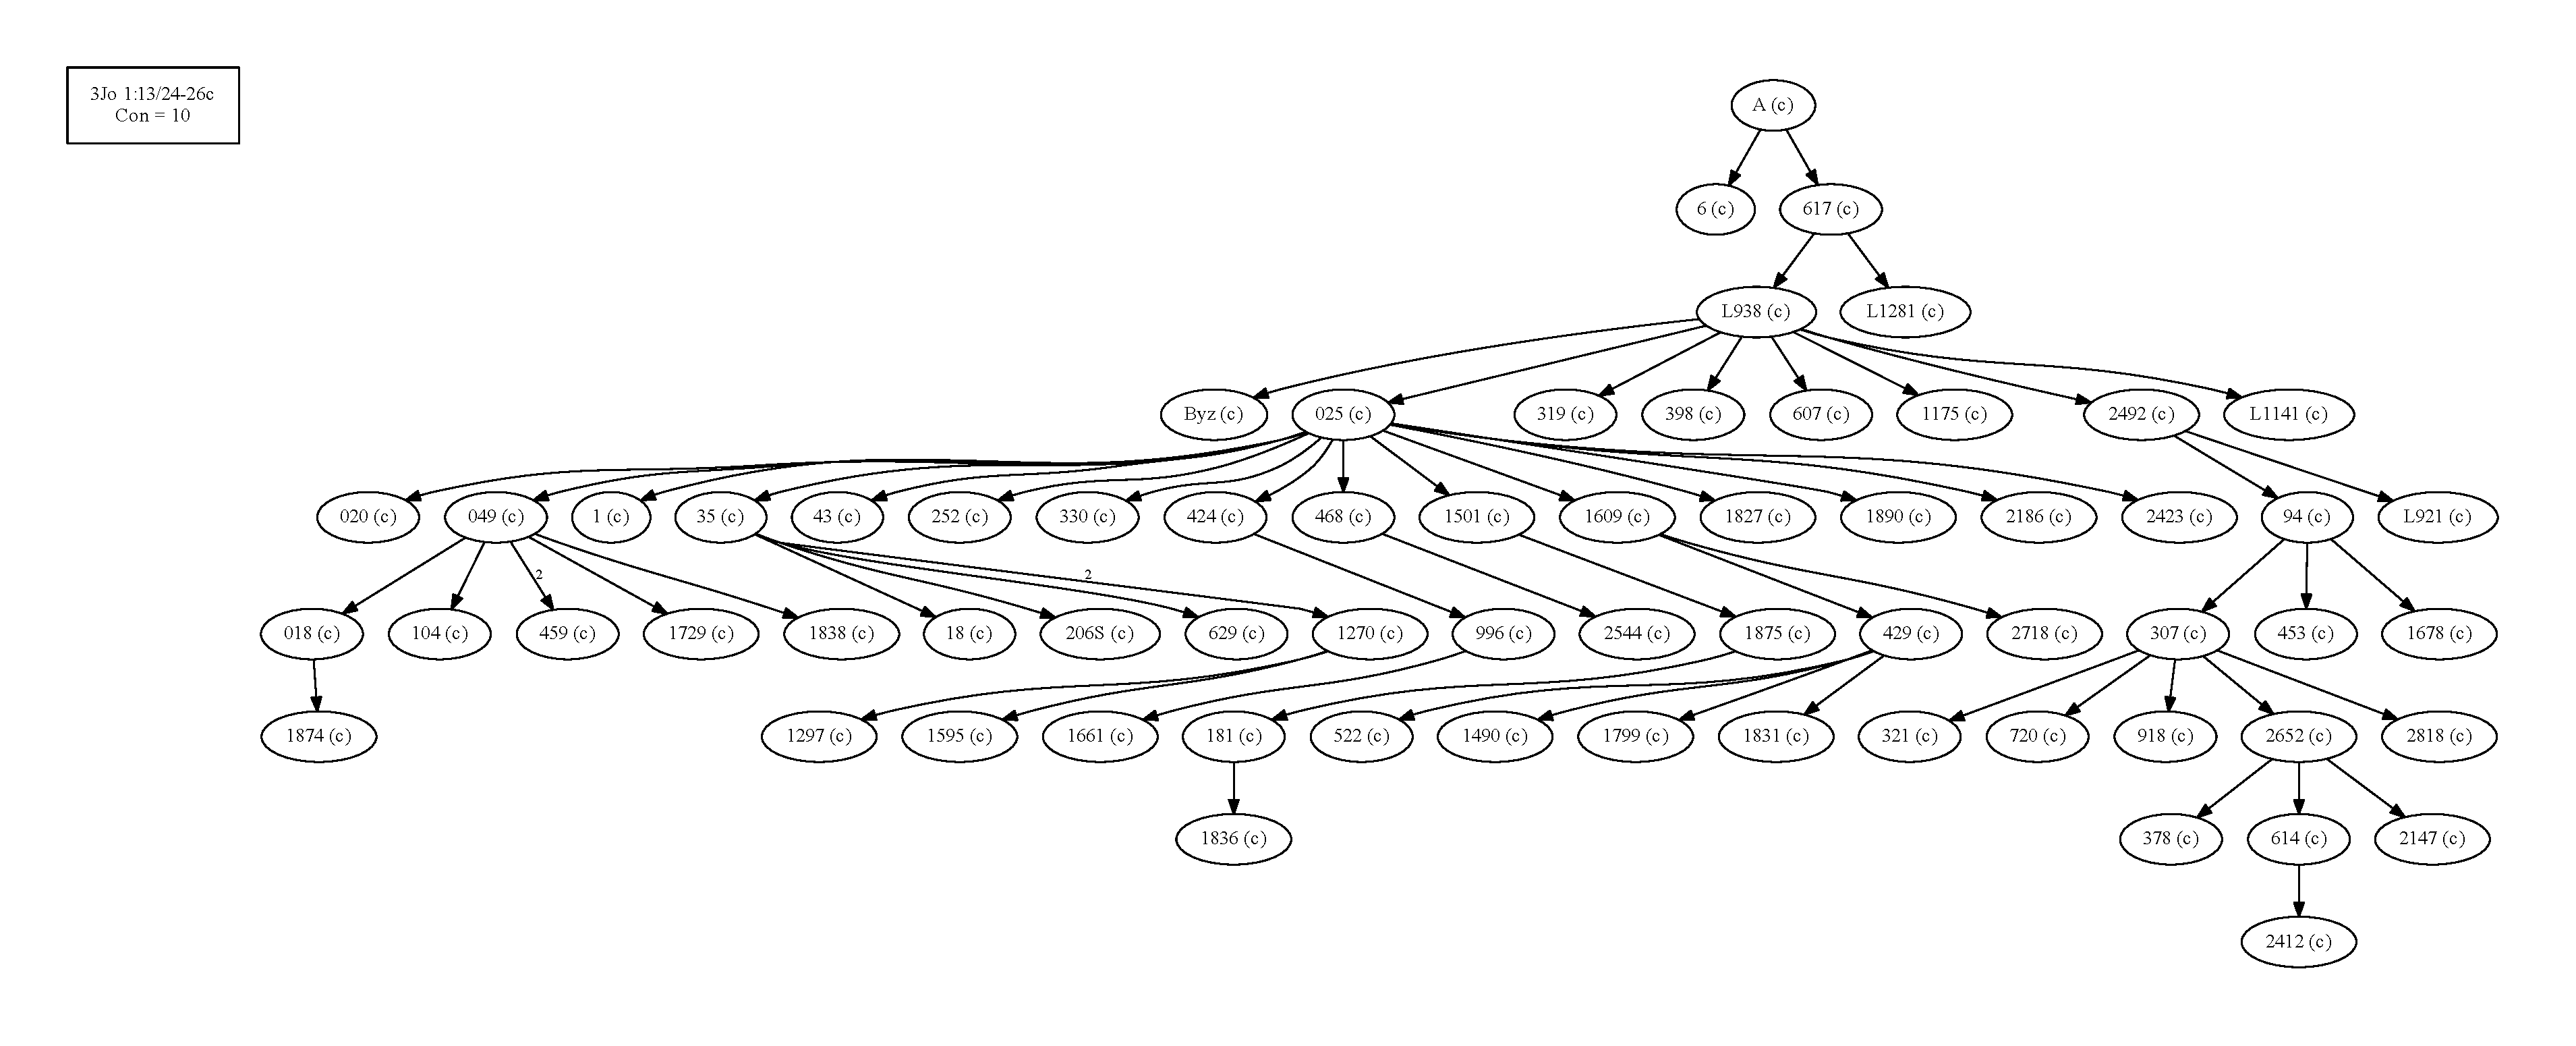
\includegraphics[scale=0.3333]{../graphics/B25K1V13U24-26Rc-coherence-attestations-3.pdf}
		\caption{Coherence in attestations diagram for 3~John 1:13\ForwardSlash 24–26, reading \emph{c}, with \emph{c} assumed to be the initial reading.}
		\label{fig:coherence-c-3}
	\end{sidewaysfigure}
	
	\newpage
	
	\subsection{Revising Local Stemmata}\label{subsec:revising-local-stemmata}
	To tarry just a bit longer on the example of 3~John 1:13\ForwardSlash 24–26, we will now attend to the task of filling in the incomplete parts of the local stemma. Recall that in the stemma of Fig.~\ref{fig:genealogical-relationships}, readings \emph{e} and \emph{f} have uncertain origins and have been left disconnected from the rest of the stemma. We can develop hypotheses about the sources of readings like these using a modification of the textual flow diagram called the \emph{coherence in variant readings} diagram. This graph contains only the witnesses and textual flow edges from the complete diagram that represent changes in readings. In some implementations, like the one pictured in Fig.~\ref{fig:coherence-variants}, it also adds edges for a witness's potential ancestors of higher ranks (within the connectivity limit) if they support different readings than its first potential ancestor. This gives the textual critic a more comprehensive picture of the possible sources of a given reading.
	
	As Fig.~\ref{fig:coherence-variants} makes clear, a witness may have several potential ancestors with distinct readings, even within a small connectivity limit. To make it easier to distiguish and weigh these possibilities, we can highlight the \emph{stability} of each textual flow from an ancestors to its descendent, defined as the number of prior readings in the ancestor minus the number of posterior readings in the ancestor, all taken as a proportion of the number of passages in which both the ancestor and descendant are extant.\footnote{This suggestion has been made by \cite[55--57]{Mink04} and \cite[273--279]{Edmondson19}.} The intuition is that a more stable textual flow is a more consistent and reliable indication of the source of a reading. A coherence in variant readings diagram with stability of textual flow highlighted in presented in Fig.~\ref{fig:coherence-variants-strengths}.
	
	\newpage
	
	\begin{figure}[h!]
		\centering
		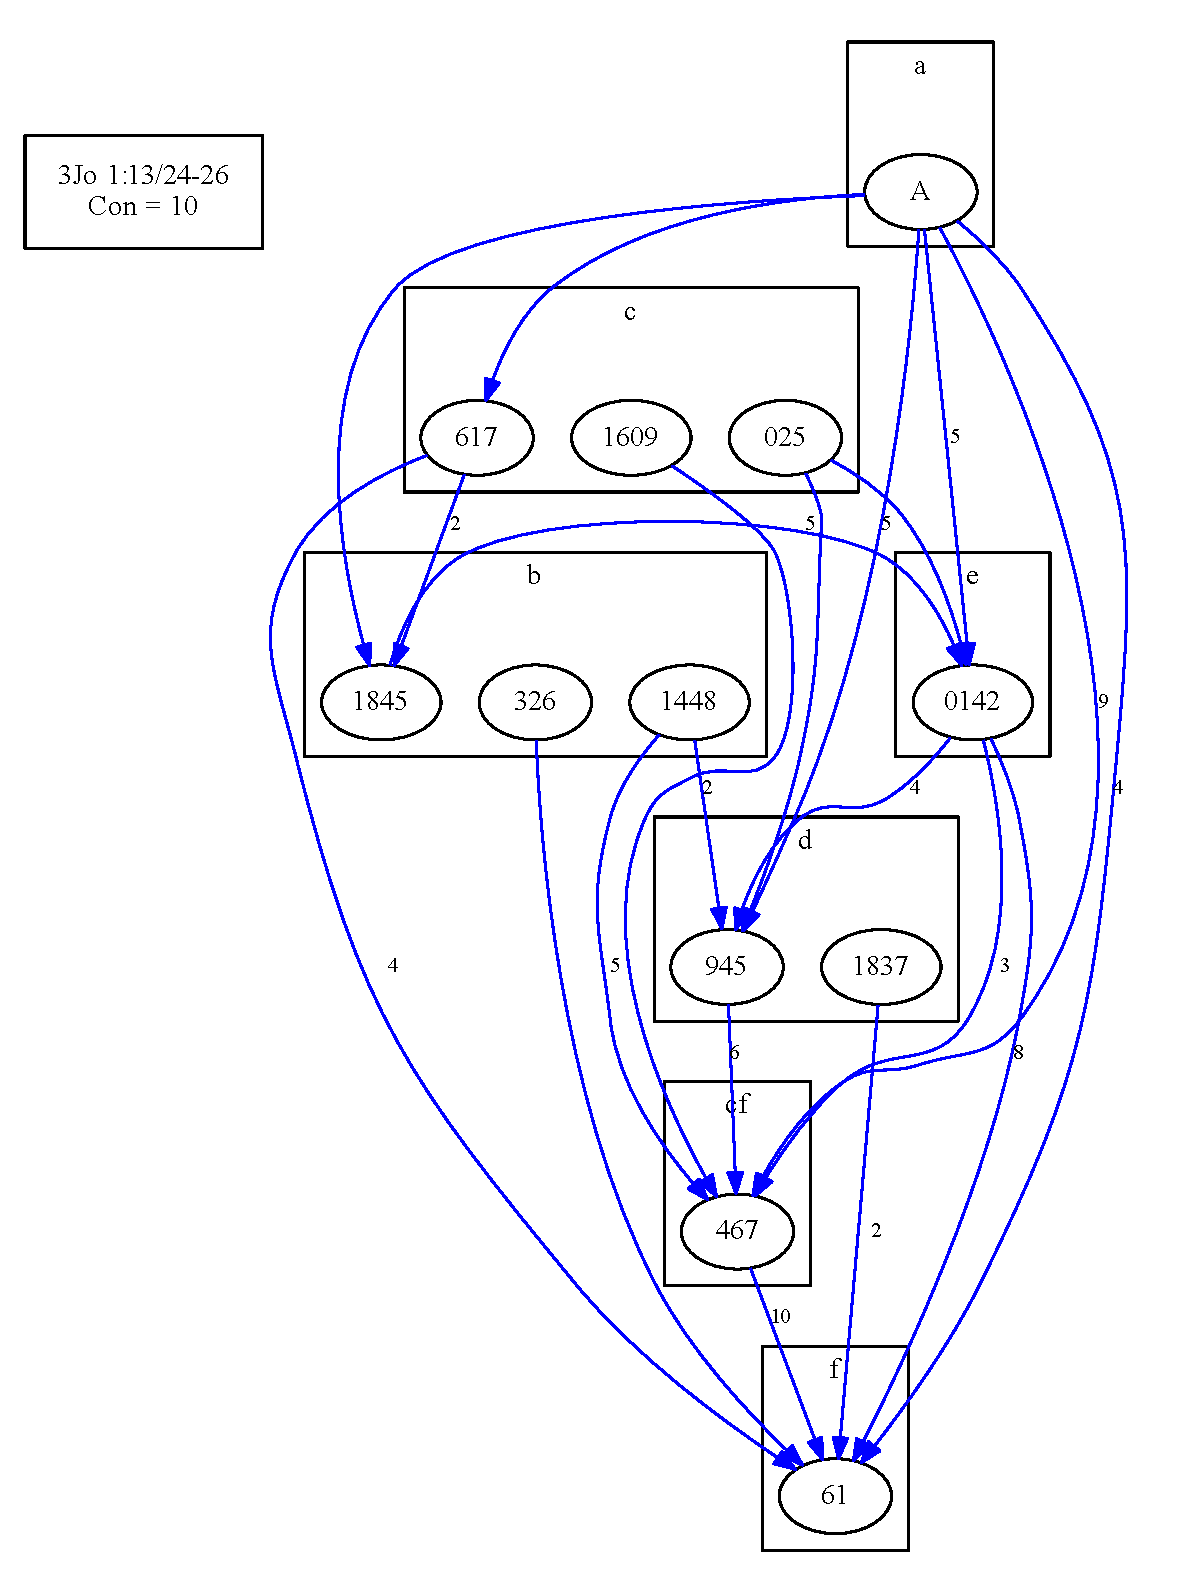
\includegraphics[scale=0.65]{../graphics/B25K1V13U24-26-coherence-variants.pdf}
		\caption{Coherence in variant readings diagram for 3~John 1:13\ForwardSlash 24–26. Unlabeled edges reflect textual flow to a witness from its rank-1 (i.e., closest) potential ancestor; labeled edges indicate that the potential ancestor has a higher rank (and is therefore less similar to the witness).}
		\label{fig:coherence-variants}
	\end{figure}
	
	\newpage
	
	\begin{figure}[h!]
		\centering
		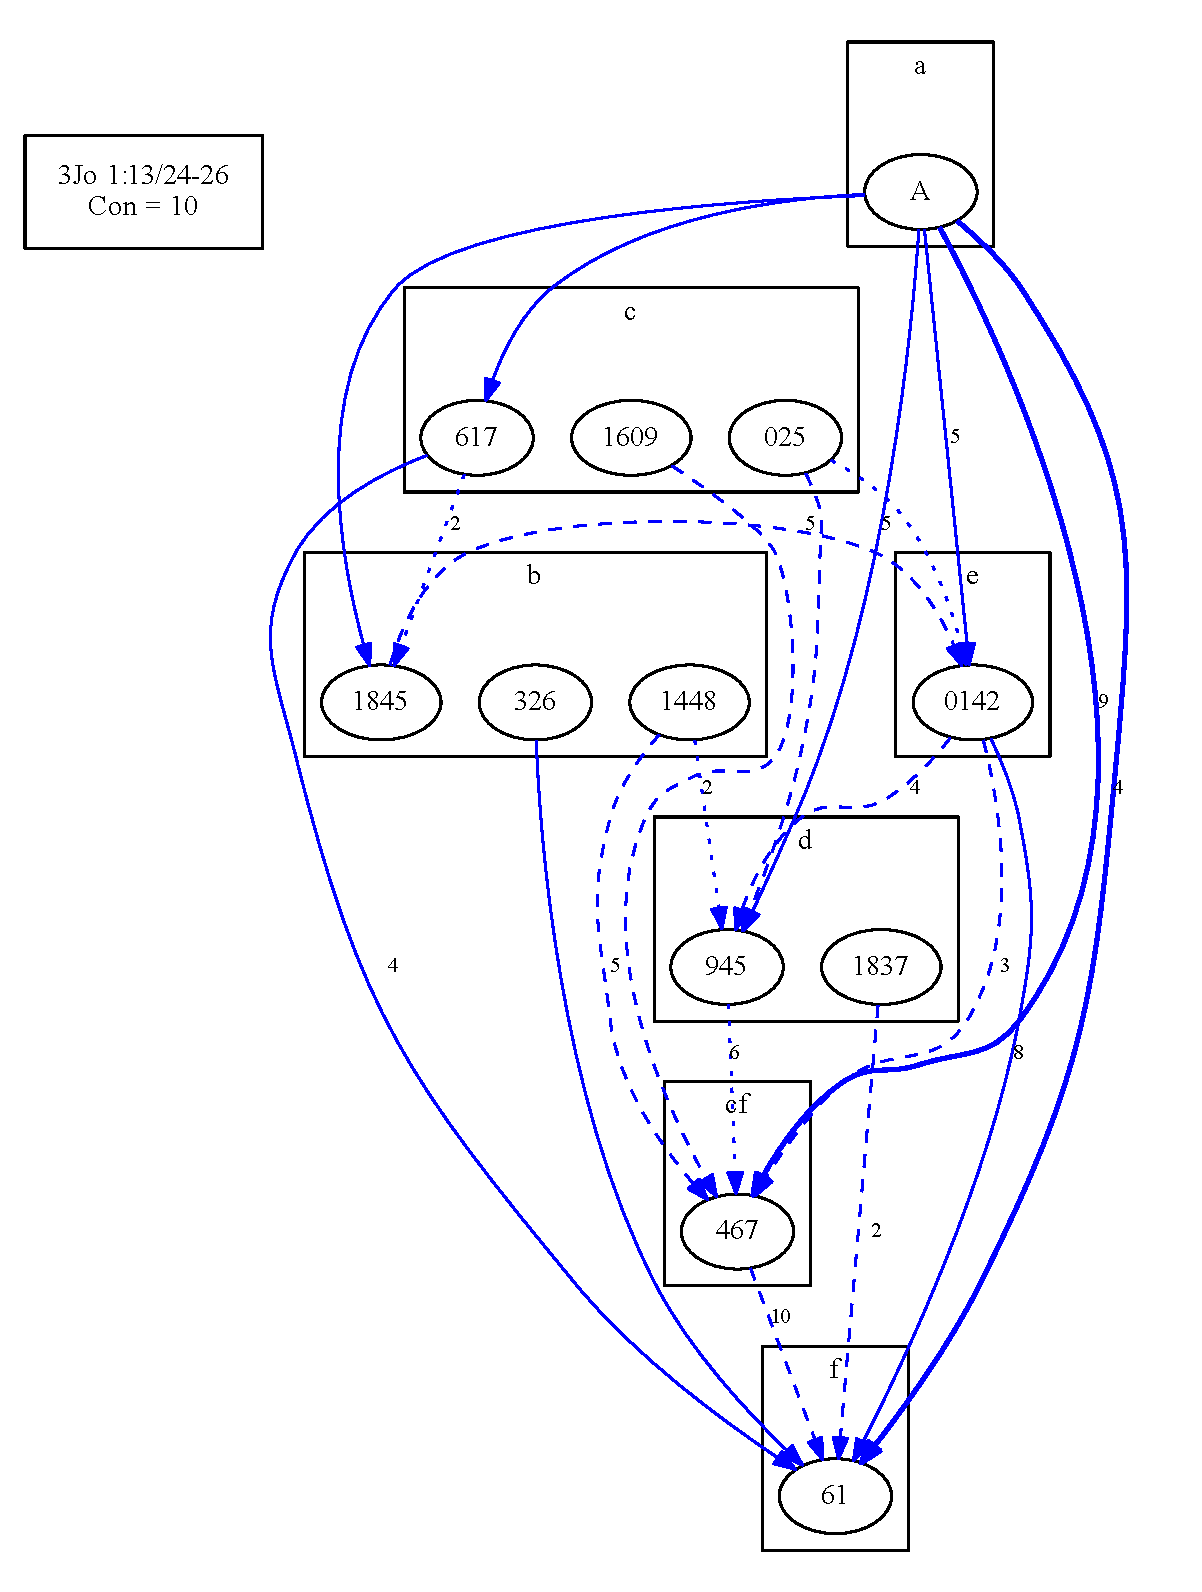
\includegraphics[scale=0.65]{../graphics/B25K1V13U24-26-coherence-variants-strengths.pdf}
		\caption{Coherence in variant readings diagram for 3~John 1:13\ForwardSlash 24–26 with stability of textual flow highlighted. Textual flow edges with stability of less than 1\% are dotted; those with stability between 1\% and 5\% are dashed; those with stability between 5\% and 10\% are solid; and those with stability of at least 10\% are bold.}
		\label{fig:coherence-variants-strengths}
	\end{figure}
	
	\newpage
	
	It is relatively easy to develop a hypothesis on the origin of reading \emph{e}. On internal grounds, the content of the reading (γραψαι) suggests that it resulted from the omission of the small word σοι in reading \emph{c} or reading \emph{d}. It turns out that within a connectivity limit of κ = 10, there is no textual flow from \emph{d} to \emph{e}, so reading \emph{c} appears to be the most likely source of the reading. This dovetails with the observation that none of GA 0142's potential ancestors supports any reading other than \emph{c} until we get to the rank-5 ancestors \emph{A} (with reading \emph{a}) and GA 1845 (with reading \emph{b}). This also suggests that the instability of the textual flow from GA 025 to 0142 in Fig.~\ref{fig:coherence-variants-strengths} is due to the high level of agreement between these witnesses (and, more broadly, the mass of surviving witnesses that support reading \emph{c}), which the table in Fig.~\ref{fig:find-relatives-0142-B25K1V13U24-26} confirms.
	
	Identifying the source of reading \emph{f} is more difficult. Within the connectivity limit, GA 61 has potential ancestors supporting every other reading, and the textual flow to 61 from most of these witnesses is stable. As the table in Fig.~\ref{fig:find-relatives-61-B25K1V13U24-26} shows, even the closest potential ancestors of GA 61 have relatively low levels of agreement with it, so stability in textual flow is more significant here than it was for GA 0142. In light of these considerations, the most likely source of the omission of reading \emph{f} seems to be reading \emph{b}, as most of GA 61's closest relatives (including its closest potential ancestor, GA 326) attest to the reading, and the textual flow from 61 to 0142 is stable.
	
	\begin{figure}[h!]
		\centering
		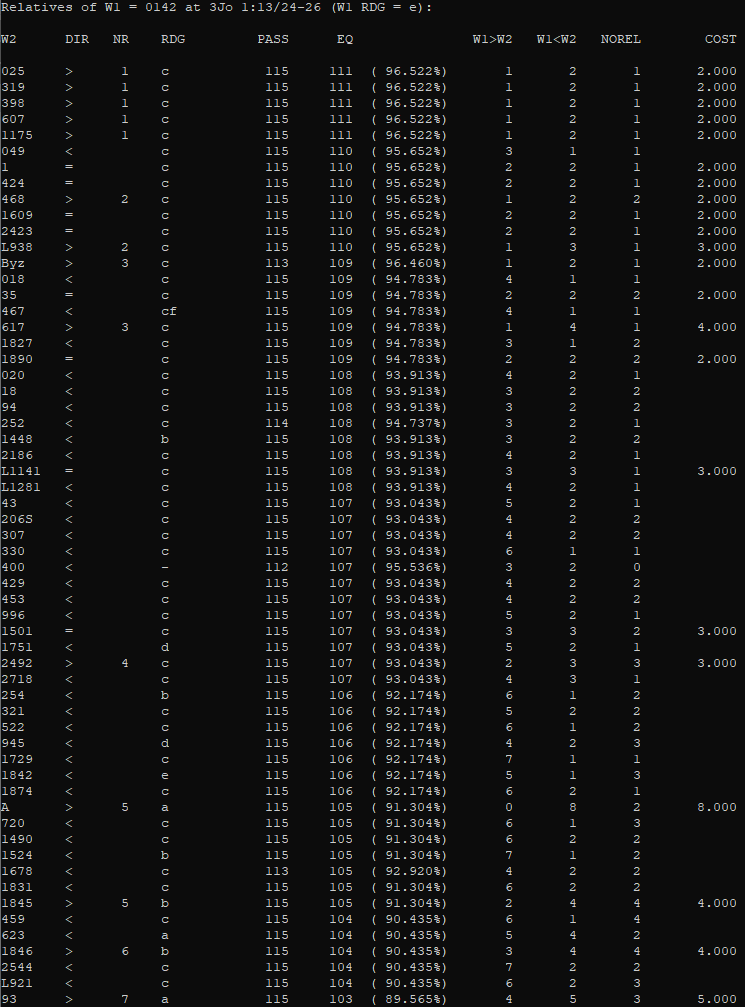
\includegraphics[width=\textwidth]{../graphics/find-relatives-0142-B25K1V13U24-26.png}
		\caption{Table of closest relatives to GA 0142 in 3~John 1:13\ForwardSlash 24–26.}
		\label{fig:find-relatives-0142-B25K1V13U24-26}
	\end{figure}
	
	\newpage
	
	\begin{figure}[h!]
		\centering
		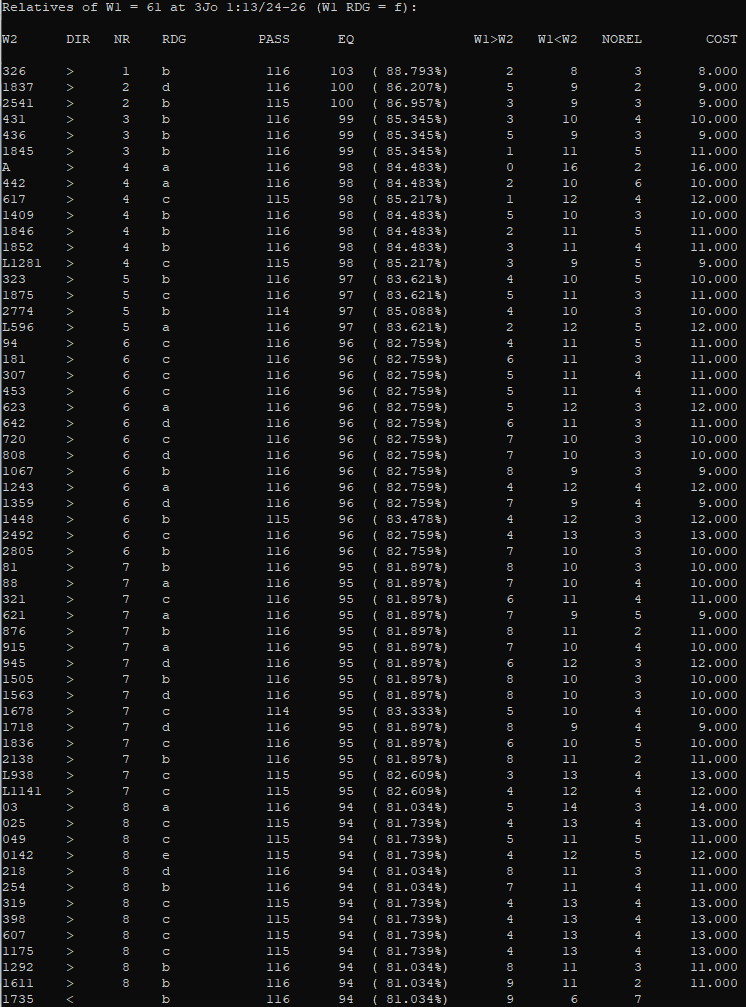
\includegraphics[width=\textwidth]{../graphics/find-relatives-61-B25K1V13U24-26.png}
		\caption{Table of closest relatives to GA 61 in 3~John 1:13\ForwardSlash 24–26.}
		\label{fig:find-relatives-61-B25K1V13U24-26}
	\end{figure}
	
	\newpage
	
	Having made these judgments, we can revise the local stemma for this passage to the complete local stemma pictured in Fig.~\ref{fig:local-stemma-completed}.
	
	\begin{figure}[h!]
		\centering
		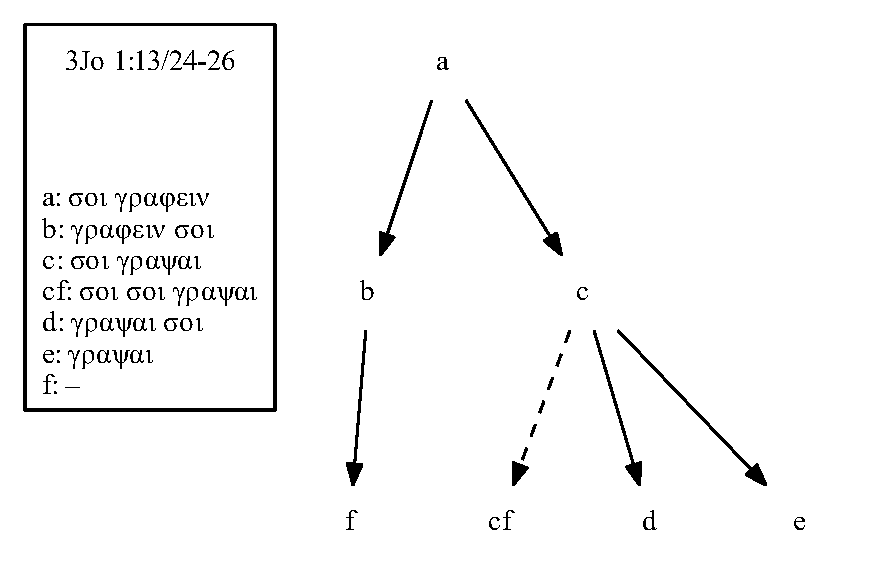
\includegraphics[scale=0.6666]{../graphics/B25K1V13U24-26-local-stemma-completed.pdf}
		\caption{Completed local stemma of 3~John 1:13\ForwardSlash 24–26.}
		\label{fig:local-stemma-completed}
	\end{figure}
	
	\newpage
	
	\section{The Global Stemma}\label{sec:global-stemma}
	As we stated in Section \ref{sec:local-stemmata}, a desirable goal in using the CBGM is to have complete local stemmata for all variant passages in the text. In Section \ref{sec:textual-flow}, we showed how we can approach this goal by using textual flow diagrams to refine local stemmata. By iteratively repeating this process, calculating genealogical relationships and textual flows between witnesses using local stemmata and then using textual flow relationships to update local stemmata, we can converge on a set of complete local stemmata in which every variant reading is explained. Once we have done this, we are ready to construct the \emph{global stemma}, a representation of textual history in terms of abstract states of the text (i.e., witnesses) in which every variant reading is explained according to the relationships encoded in local stemmata.\footnote{There has been some debate over the extent to which the CBGM can reconstruct textual history. Shorter treatments of this topic can be found in \cite{Wachtel15} and \cite{Carlson15}. An evaluation of the CBGM against more traditional stemmatic methods believed to better-suited to the reconstruction of a tradition's history can be found in \cite{Edmondson19}. A more recent and rigorous critique of the method's approach to reconstructing textual history can be found in \cite{Carlson20}.}
	
	A global stemma bears a superficial similarity to a textual flow diagram, in that both structures connect potential ancestors and descendants based on their genealogical relationships, but it differs in the following respects:
	\begin{itemize}
		\item A textual flow diagram is constructed for a specific passage, and connectivity is determined exclusively by the variant readings in that passage; a global stemma is constructed with all passages in mind (thus making it \emph{global}).
		\item As a consequence of the previous distinction, a textual flow diagram need not concern itself with contamination, or a witness's derivation of readings from multiple sources, while a global stemma by design must account for contamination wherever it may have occurred. To speak in more functional terms, a textual flow diagram assigns each witness at most one textual flow ancestor, while a global stemma can assign a witness multiple ancestors.
		\item A textual flow diagram can extrapolate reading relationships that are inconsistent with local stemmata, while the structure of a global stemma is constrained by the structure of local stemmata. That is, in a textual flow diagram for a given passage, textual flow may pass between witnesses with readings that have no relationship in the local stemma for the same passage (as we showed for readings \emph{e} and \emph{f} in Subsection \ref{subsec:revising-local-stemmata}), while in a global stemma, every reading attested by a witness must be explained by at least one of its ancestors according to the local stemma of the associated passage.\footnote{It is worth noting that not all implementations of the CBGM make this last distinction. In \cite{Edmondson19}, for instance, textual flow relationships where the reading changes from textual flow ancestor to textual flow descendant are only allowed to occur when the ancestor's reading is directly prior to the descendant's reading in the local stemma. This results in textual flow diagrams that are far more consistent with the global stemma, but it also inhibits the use of the textual flow diagram as a tool for confirming or refuting hypotheses about variant readings.}
	\end{itemize}
	
	\newpage
	
	\subsection{Substemmata of Witnesses}\label{subsec:substemmata}
	Like a textual flow diagram, a global stemma can be constructed witness-by-witness. We refer to the portion of a global stemma containing a witness and its ancestors as that witness's \emph{substemma}. The procedure of determining the best choice of stemmatic ancestors for a given witness is called \emph{substemma optimization}, and it is both more complicated and more reliant on human input than its counterpart for textual flow diagrams. We will attempt to elucidate the process by means of illustrations and examples.
	
	In substemma optimization, the readings of a witness are compared to the readings of a potential ancestor at every passage where the witness has a surviving reading. We say that the witness's reading is \emph{explained} by the potential ancestor's reading if both readings agree or if the potential ancestor's reading gives rise to the witness's reading in local stemma for that passage.\footnote{In most formulations of the CBGM, the second condition is interpreted to mean that the potential ancestor's reading is \emph{directly} prior to the witness's reading. The constraint formulated this way is precise, but as \cite[59--63]{Mink04} and \cite[139--140]{Edmondson19} have pointed out, its strictness can produce unavoidable gaps in the global stemma that can only be resolved in an ad hoc manner. The \textsf{open-cbgm} library avoids this problem by relaxing the constraint so that any reading prior to a witness's reading explains it.} This principle is illustrated in Fig.~\ref{fig:explained-readings}.
	
	\begin{figure}[h!]
		\centering
		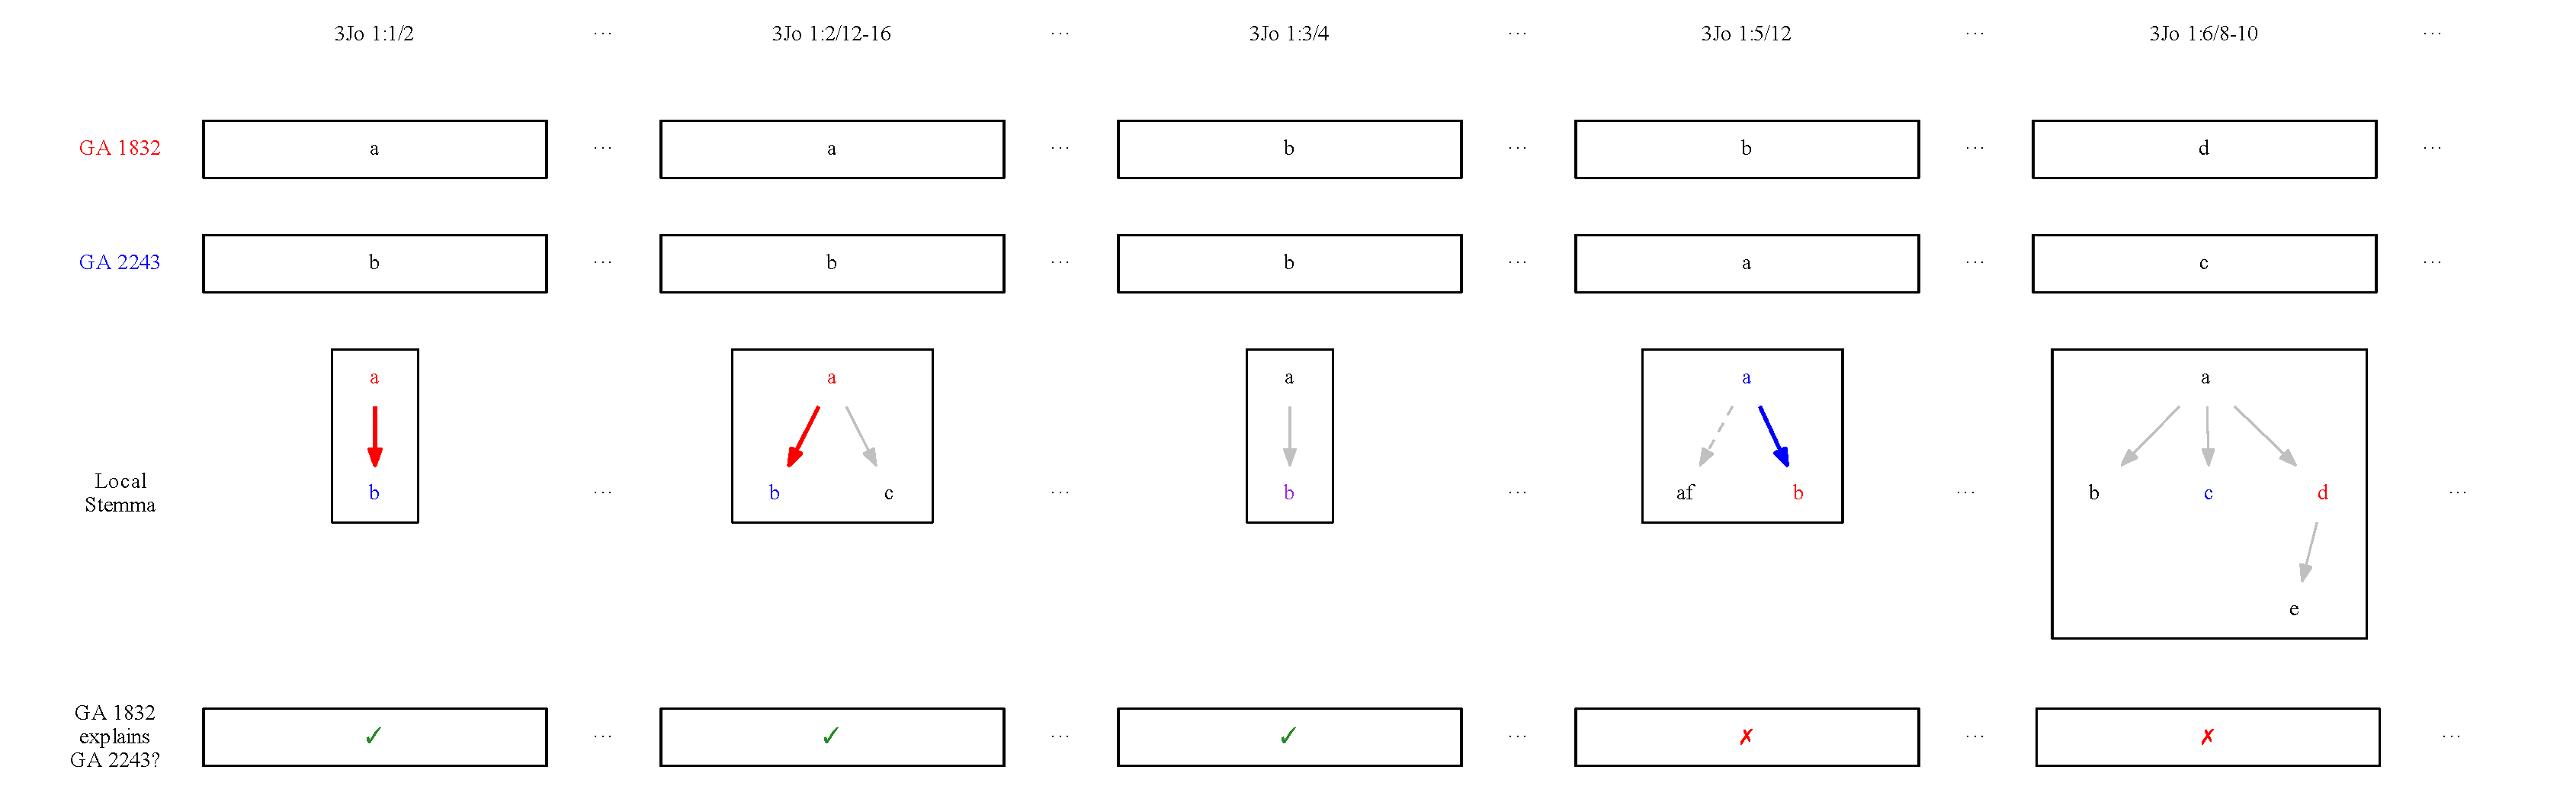
\includegraphics[width=\textwidth]{../graphics/explained-readings.pdf}
		\caption{Illustration of a comparison (at selected passages) between a witness (GA 2243) and a potential ancestor (GA 1832) for substemma optimization. In the first two example passages, 1832's reading explains 2243's reading by priority. In the third, 1832's reading explains 2243's reading by agreement. In the fourth, 1832's reading does not explain 2243's reading because 2243 is prior to 1832 here. In the fifth, the two witnesses' readings have no relationship, so 1832's reading does not explain 2243's reading. This means that if 1832 is a stemmatic ancestor of 2243, then it cannot be the only one; 2243 needs another ancestor to explain any passages that 1832 cannot.}
		\label{fig:explained-readings}
	\end{figure}
	
	\newpage
	
	In many cases, it is impossible to explain all of a witness's readings using a single ancestor. When this happens, we assume that \emph{contamination} or mixture of readings from different exemplars has occurred in the copying process, and we must find a substemma with multiple ancestors such that every reading in the witness is explained by at least one of its ancestors. In the example in Fig.~\ref{fig:explained-readings}, the readings of GA 2243 cannot be explained by a substemma consisting of just GA 1832, but if we add GA 2544 to the substemma, then every reading in 2243 is covered (see Fig.~\ref{fig:contamination}).
	
	\begin{figure}[h!]
		\centering
		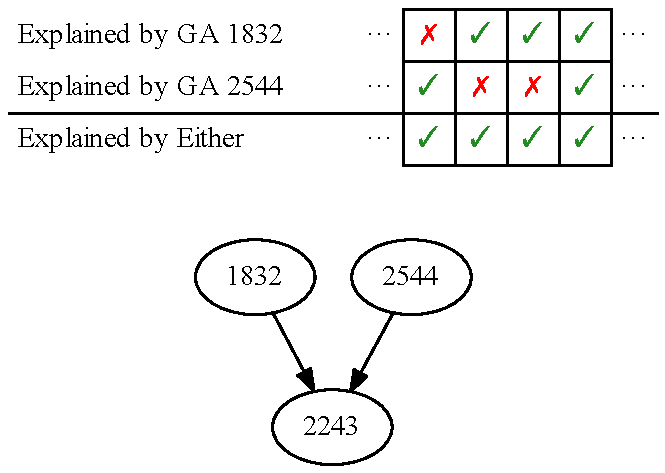
\includegraphics[scale=0.6666]{../graphics/contamination.pdf}
		\caption{Accounting for contamination in the substemma for GA 2243. Top: explained reading arrays for selected passages between 3~John 1:6\ForwardSlash 8–10 and 3~John 1:6\ForwardSlash 24–28 for potential ancestors of 2243 and the combined array for the substemma consisting of those ancestors. Bottom: graphical representation of the substemma.}
		\label{fig:contamination}
	\end{figure}
	
	In practice, a witness may have multiple \emph{feasible} substemmata that explain all of its surviving readings (see Fig.~\ref{fig:substemmata}), but we want to find one that is \emph{optimal} in some measureable sense. The closest thing we have to official criteria to this end are two of the CBGM's methodological assumptions: \emph{parsimony} (``scribes tended to use fewer sources rather than many'') and \emph{fidelity} (``scribes tended to copy faithfully rather than innovate'').\footnote{\cite[98--99]{WG17}.} Both of these concepts can be associated with objective, measureable quantities (the number of ancestors in a substemma and the pre-genealogical similarities between the descendant and its ancestors in the substemma, respectively), but there is no obvious way to optimize them jointly. A two-ancestor substemma is more parsimonious than a three-ancestor substemma, but the additional third ancestor may explain many more of the descendant's readings by agreement, which coheres better with the assumption of fidelity. It is therefore incumbent upon the textual critic to make informed judgments about competing substemmata by weighing parsimony, levels of agreement, and external philological factors accordingly.
	
	\begin{figure}[h!]
		\centering
		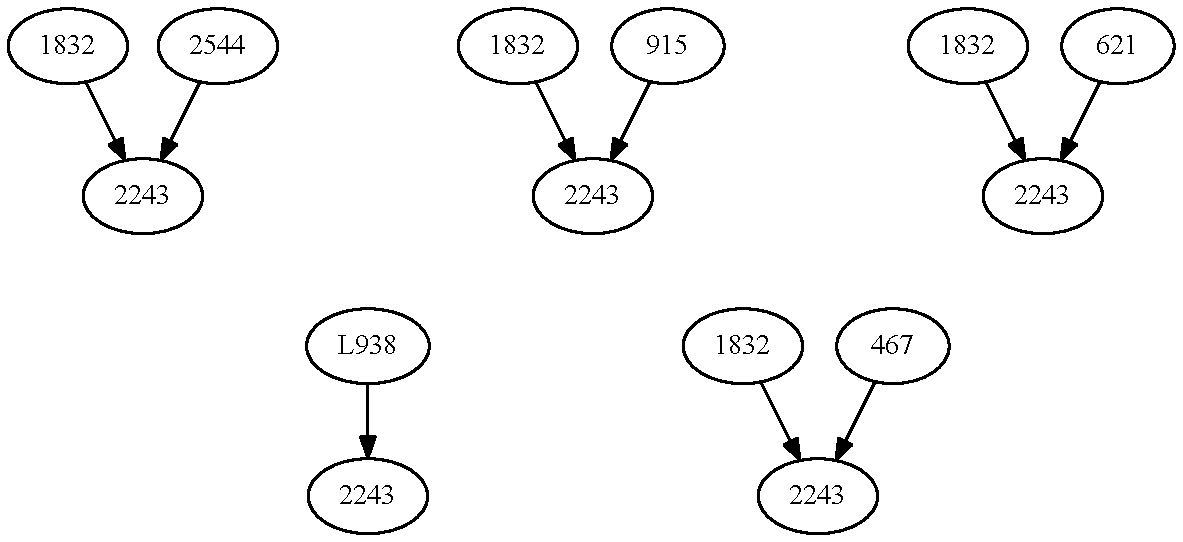
\includegraphics[scale=0.6666]{../graphics/substemmata.pdf}
		\caption{Five of the many feasible substemmata for GA 2243 in 3~John. The fourth substemma is the most parsimonious, but it only explains ninety-seven of 2243's 107 readings by agreement. The fifth substemma, meanwhile, explains 104 out of 107 readings by agreement.}
		\label{fig:substemmata}
	\end{figure}
	
	\newpage
	
	Evaluating a single candidate substemma can be done quickly and easily, but since the number of possible substemmata for a witness with $k$ potential ancestors is $2^k -1$, the more pressing problem is to narrow down the list of candidates to a manageable number. In practice, we can usually restrict our attention to substemmata containing only the witness's closest few potential ancestors,\footnote{The CCeH implementation of the CBGM currently allows users to evaluate substemmata consisting of up to twelve potential ancestors. For twelve potential ancestors, there are $2^{12} - 1 = 4095$ substemmata.} in which case a brute-force evaluation of the substemmata for all combinations of ancestors can be done in a reasonable amount of time.
	
	Alternatively, if we have a preferred criterion of optimality by which to score substemmata, then we may be able to use known heuristics to find all feasible substemmata close to a given score without having to specify their constituent ancestors. Because substemma optimization can be shown to be a computationally difficult problem,\footnote{In its most basic form, it is an instance of the \emph{minimum set cover problem}, which belongs to the computational complexity class of \emph{NP-complete} problems. Many such problems have been identified, and while it is believed that no generally efficient procedures exist to solve them, a proof of this remains elusive. For a proof of the NP-completeness of set cover and a more technical survey of NP-complete problems and their relationships, see \cite{Karp72}.} it is possible that in the worst case, such heuristics will be as slow as the brute force approach. In the context of substemma optimization, however, they tend to find close or exact solutions quickly in practice.
	
	\newpage
	
	\subsection{Putting It All Together}
	Once we have performed substemma optimization for every witness, we can combine all of our best-found stemmatic ancestor-descendant relationships into a complete global stemma. The result should be a fully connected graph detailing witnesses' sources and any contamination between them, with the initial text \emph{A} as the unique root of the graph from which every other witness can be reached by some path.
	
	We say that the result \emph{should} be fully connected, because certain conditions must be met for this to happen. One of these conditions, as we mentioned in the beginning of Section \ref{sec:global-stemma}, is that all local stemmata should be completed, with none of their readings left unexplained. Several of the local stemmata in the ECM of 3~John were left incomplete, so in the interest of presenting a global stemma under the specified conditions, we constructed our examples in Subsection \ref{subsec:substemmata} using a modified collation where variant passages containing any readings with uncertain sources (such as 3~John 1:13\ForwardSlash 24–26) were removed. (Ideally, we would fill in the gaps of all incomplete stemmata as we did in Subsection \ref{subsec:revising-local-stemmata}, but for the sake of time, we have taken this shortcut.)
	
	Another condition for the global stemma to be connected is that there are no fragmentary witnesses that agree with the initial text \emph{A} at all of their extant passages. If such witnesses are included, then they will have equal priority to \emph{A} and will end up forming parallel ``roots'' to the global stemma. This can easily be remedied by excluding witnesses from consideration if they have fewer extant passages than a reasonable threshold. In 3~John, where we have 116 variant passages, a threshold of 100 is more than sufficient.
	
	In reality, nothing prevents us from constructing an incomplete global stemma if these conditions are not met. A global stemma constructed from a collation that includes incomplete local stemmata and fragmentary witnesses is shown in Fig.~\ref{fig:global-stemma-incomplete}. But since we want the most accurate approximation of textual history we can get, a complete global stemma is obviously preferable. Using our modified dataset that drops fragmentary witnesses and ignores passages with incomplete local stemmata, we can get a complete global stemma (see Fig.~\ref{fig:global-stemma}).
	
	\begin{sidewaysfigure}
		\centering
		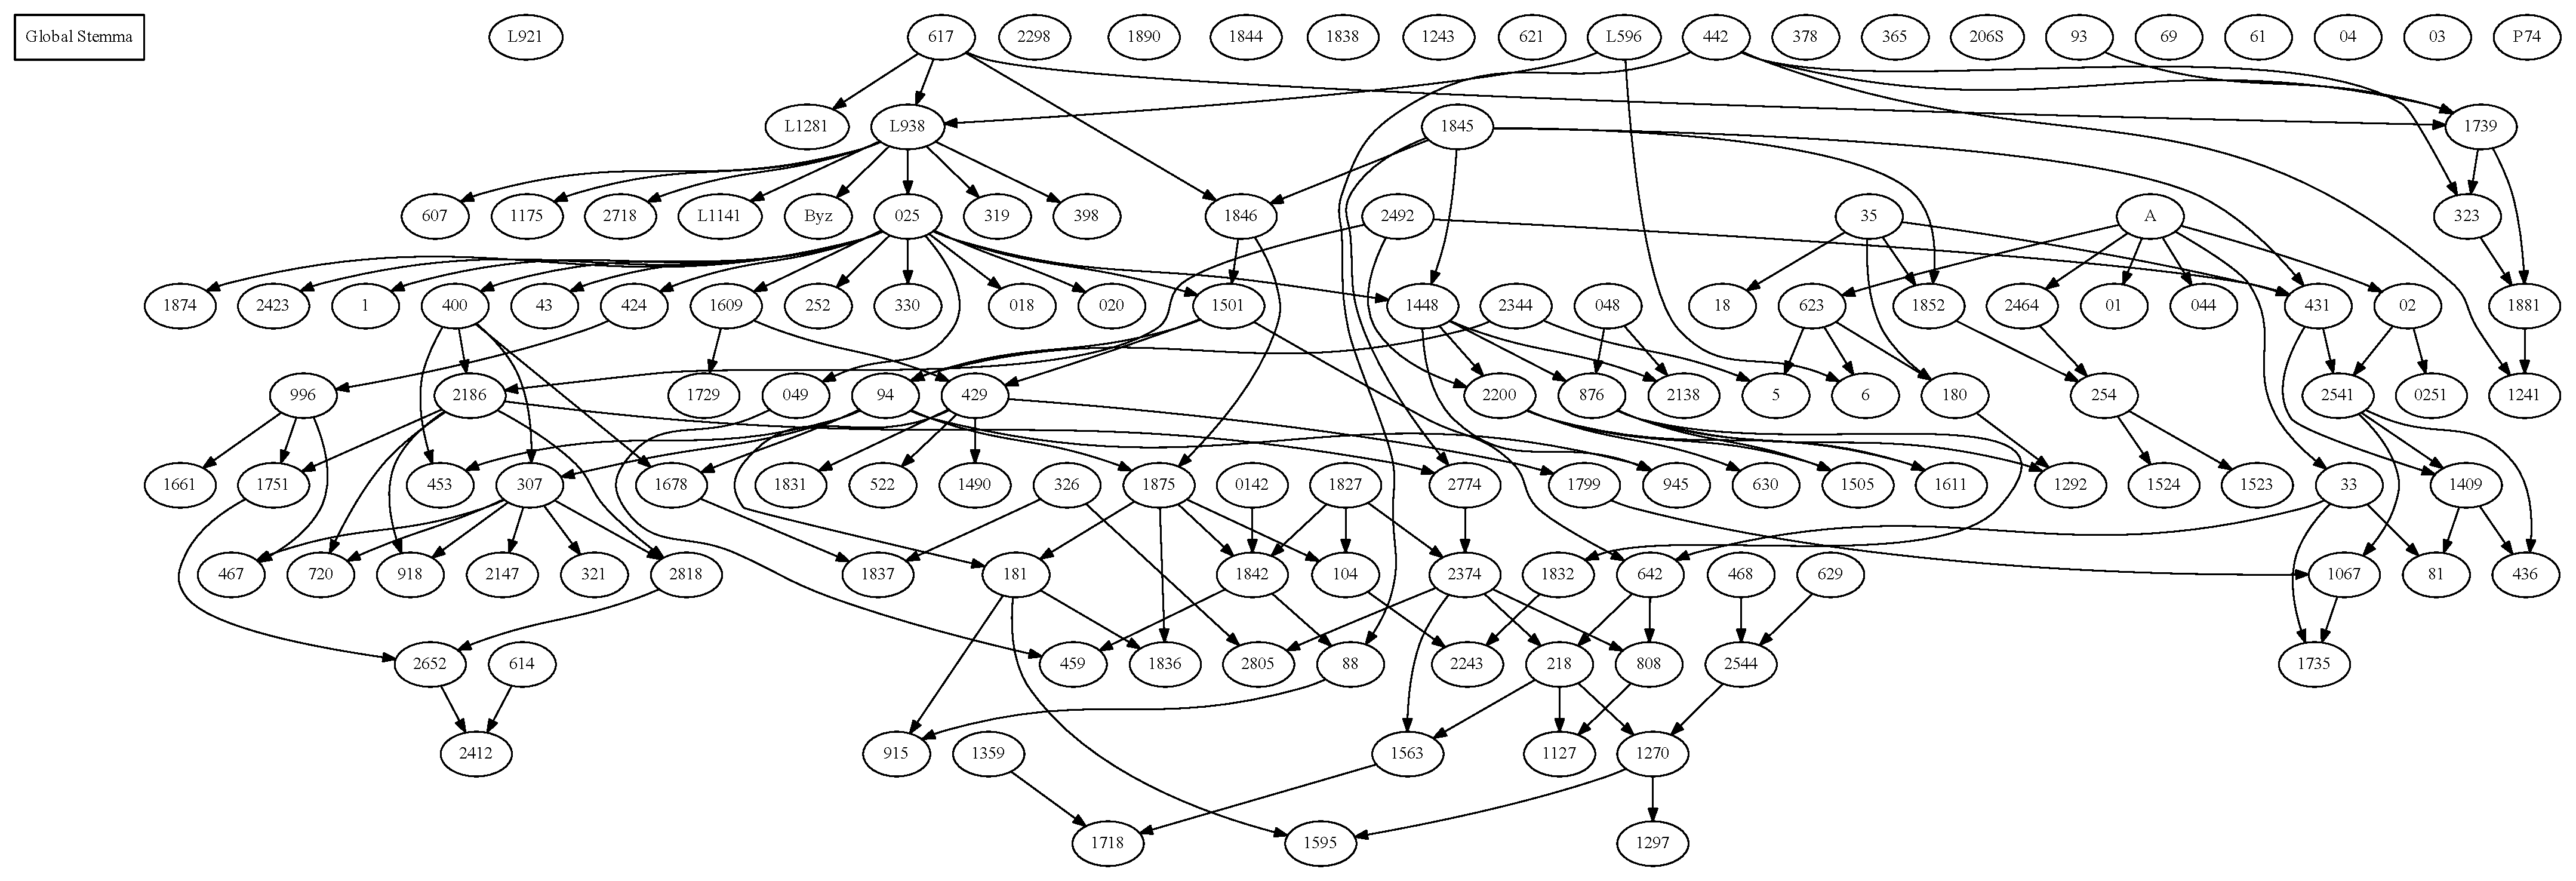
\includegraphics[width=\textwidth]{../graphics/global-stemma-incomplete.pdf}
		\caption{Incomplete global stemma for 3~John. The multiple roots of the stemma are either the result of unexplained readings in local stemmata (e.g., GA 03) or fragmentary witnesses that have equal priority to the initial text \emph{A} (e.g., GA \Pap{74} and GA 365).}
		\label{fig:global-stemma-incomplete}
	\end{sidewaysfigure}
	
	\begin{sidewaysfigure}
		\centering
		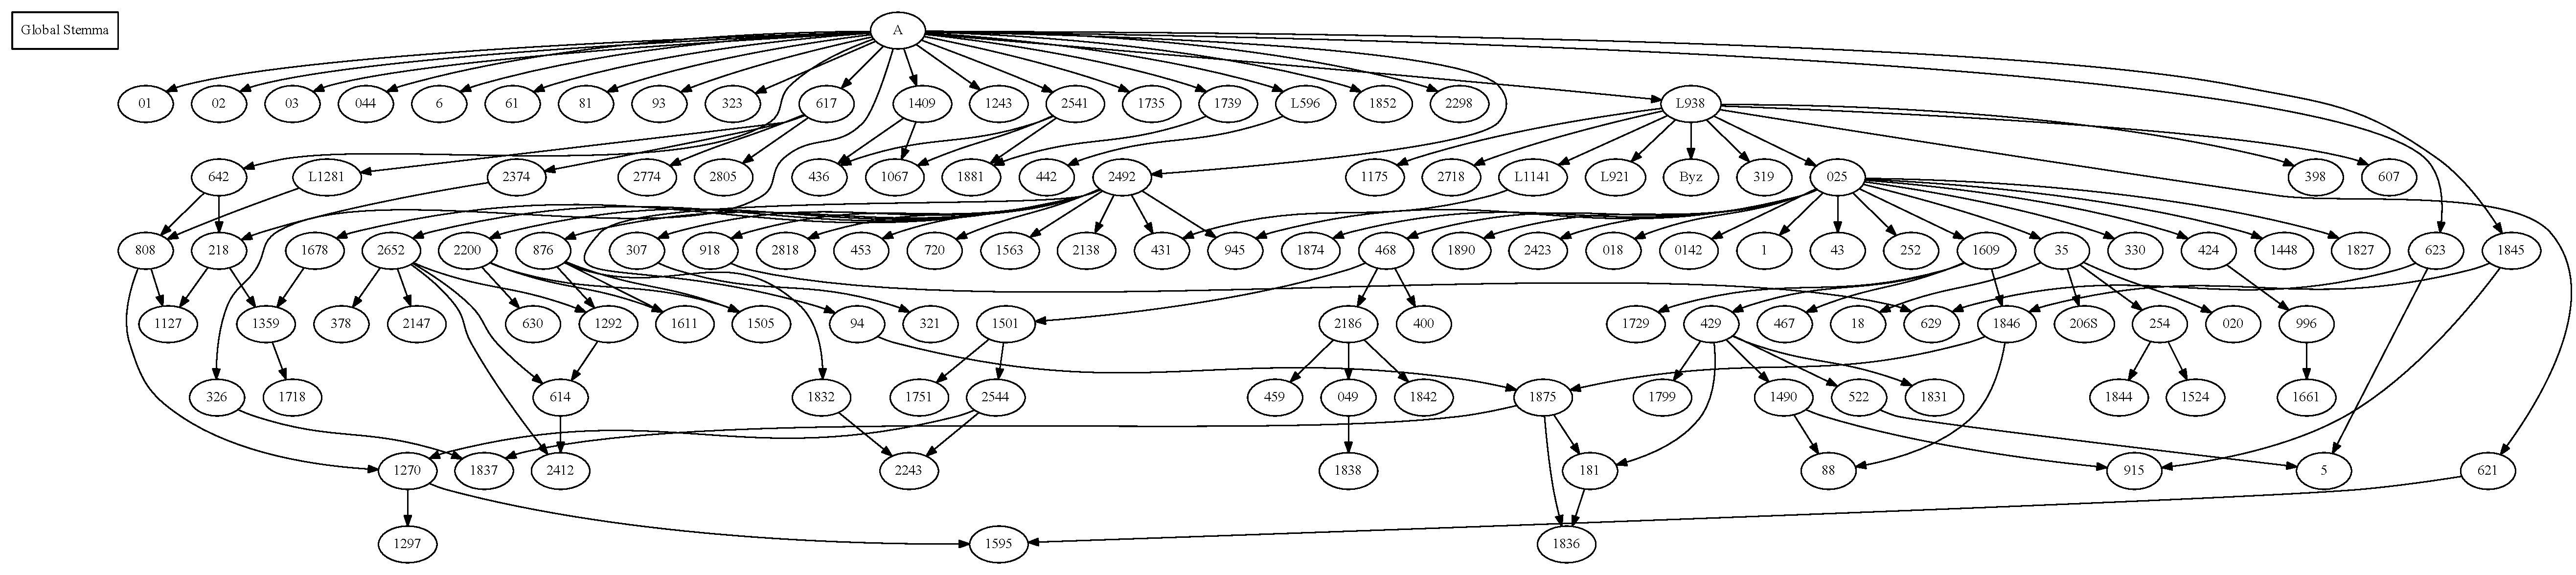
\includegraphics[width=\textwidth]{../graphics/global-stemma.pdf}
		\caption{Complete global stemma for 3~John. Note that this is a preliminary output from an automated procedure in the \textsf{open-cbgm} library. Some of the substemmata would likely change if we properly completed incomplete local stemmata instead of ignoring them, and even more would change if we incoporated our own text-critical judgments into the process of substemma optimization.}
		\label{fig:global-stemma}
	\end{sidewaysfigure}
	
	\newpage
	
	\section*{Conclusion}\label{sec:conclusion}
	This concludes our crash course on the CBGM. My primary intention for this (relatively) short illustration- and example-driven document was to provide prerequisite knowledge about the CBGM for my 2020 SBL Annual Meeting talk on the \textsf{open-cbgm} software library, but I hope that it can outlive this more immediate purpose to serve as a general guide on the basics of the method. To reiterate comments made in the introduction, the reader interested in learning more is recommend to consult the introductions cited in the introduction, as well as any of the works cited in the References section.
	
	\printbiblist{abbreviations}
	\printbibliography
\end{document}